
\chapter{Dynamic Component Model}

This chapter describes our solution to the problem of extending U-Sem by adding custom functionality. Section \ref{sec:problemDef} identifies the problem in details and describes all functional and non-functional requirements that a successful solution must satisfy. Section \ref{sec:approach} discusses that state of the art approaches and technologies that  can be used to solve the problem. Section \ref{sec:architecture} describes the extension of the architecture of U-Sem that we provide in order to solve the problem. Section \ref{sec:impl} briefly discusses the simple implementation that we provide in order to be able to verify the capabilities of the architecture we propose. Section \ref{sec:eval} discusses and verifies whether the proposed solution satisfies all of the requirements. Finally, in section \ref{sec:limits} we discuss the limitations of the proposed design and suggests aspects in which the design can be improved in the future.


\section{Problem definition}
\label{sec:problemDef}

During the initial interviews with the potential scientists that are going to use the system, we reviled that the nature of their work is very dynamic. In their day to day work they are expected to constantly improve and come up with new algorithms and approaches for user modelling. As a result, they are continuously producing new software code that implements these algorithms. After each production cycle, the program code has to be deployed into U-Sem so that it is available for testing, demonstration and evaluation purposes.

We then performed additional interviews with the scientist in order to reveal how this process is currently done, what are the problems they face with it and what are their expectations for the future system. Scientists reported that they have on their disposal only the capabilities of the workflow engine(RDFGears). However, it provides no functionality that enables to plug in custom logic on demand into the system and as a result scientists are forced to "hardcode" their logic into the source code of the workflow engine. In this way the software code implementing the algorithms becomes part of the workflow engine. We believe that this approach is error prone and brings a lot of discomfort to the scientists working with the system. The most important disadvantages of this approach include:

\begin{itemize}

	\item Adding new or modifying existing functionality requires a lot of time and knowledge since in order to do that one has to alter the source code of the workflow engine and basically release a new version of it. This process requires advanced knowledge about each phase of the release process: checking out the source code from the software repository, writing the new source code in the appropriate place, building the system and finally deploying it to the web server. Most of the time, all this knowledge is not required for the daily work of scientists and learning it creates a serious overhead and discomfort.
	
	\item In order to add/modify functionality one has to stop the web server where the system is deployed, replace the deployment entities of the system and start the server again. The problem with this approach is that during the time the server is down all other running services are unavailable. This is a major problem for everyone that is using the system during that time.
	
	\item Another major disadvantage is that as a result of all the additional knowledge required the training period for new scientists is significantly increased. This may easily cause project delays and missed deadlines.
	
	\item Multiple scientists adding/modifying functionality simultaneously may result in loss of functionality. Figure \ref{fig_vers_prob} illustrates the problematic scenario. As stated earlier in order to add new functionality scientists must first check out the source code of the system, make the changes and deploy the new version on the web server. However, if two scientist perform this process simultaneously then the new functionality provided by the first scientist will be lost when the second one deploys his version. 
	
	\begin{figure}[h!]
  \centering
  	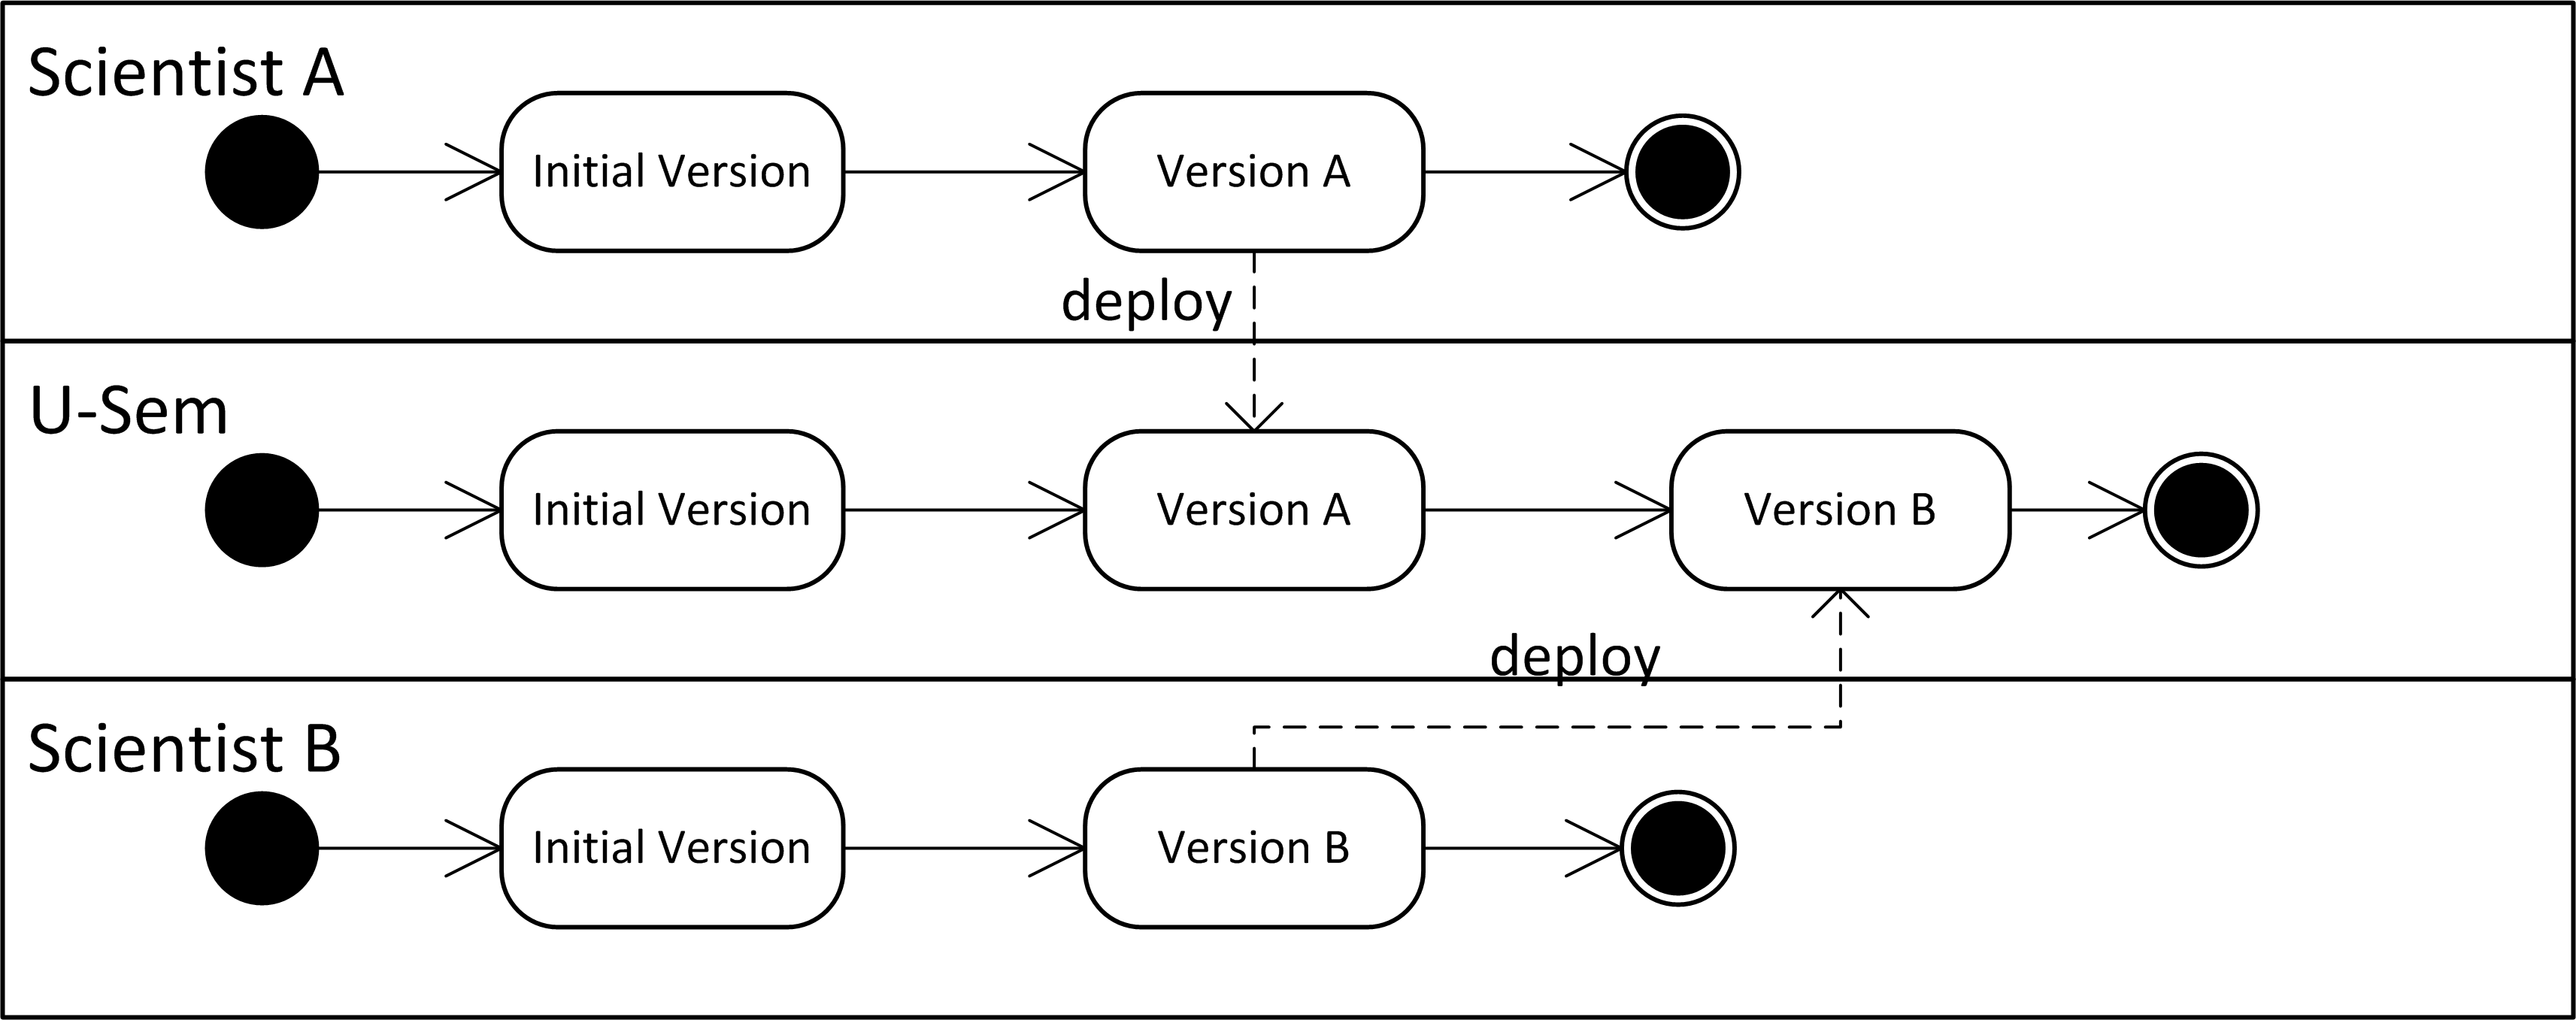
\includegraphics[scale=0.75]{plug-in/version_problem.png}
  \caption{State diagram illustrating the scenario where two scientists extend U-Sem simultaneously and the changes made by Scientist A are lost.  }
  \label{fig_vers_prob}
\end{figure}
	
	\item And last but not least, it is hard to verify what is the exact state of the system at any particular moment. Unless documented exclusively, it is not clear what additional functionality is added to the system. This problem becomes more serious when there are more people working on the project simultaneously and it is hard to track the changes in the system.
		
\end{itemize}

This approach also introduces one big disadvantage from software engineering perspective. The problem lies in the poor modularization of the system. In software engineering, modularization is considered as a key property for improving extensibility, comprehensibility, and reusability in software projects \cite{Parnas}. The most important aspect of a successful modular system is its information hiding capabilities \cite{Srivastava}. In our case, scientists can only rely on the modularization functionality provided by the Java language. However, its information hiding principles are only applied on class level, but not to the level of packages and JAR files. For example, it is not possible to restrict access to certain public classes defined in a package. The absence of such visibility control can easily lead to highly coupled, "spaghetti-like" systems \cite{Eder}. The consequences of this will become more and more clear with the time when the system grows in size, complexity and the number of engineers working on it increases. The most probable consequences include high development costs, low productivity, unmanageable software quality and high risk to move to new technology \textbf{Cai}.

Having all these considerations in mind, we devised a complete set of requirements that presents the functional scenarios(functional requirements) and system qualities(non-functional requirements) that the proposed architecture has to provide. These requirements are also referred to into the evaluation section where we discuss how and to what extend the architecture satisfies each of them.


\subsection{Functional Scenarios}
In this section we formally identify the functional requirements which define the main interactions between the scientists and the system. Each scenario is marked with a small code at the beginning which is used for easier identification during the validation and evaluation phase.

\begin{itemize}

	\item \textbf{UC1 - Adding custom functionality} - This is the main scenario regarding the feature we design in this chapter. Scientists has to be able to extend U-Sem by adding custom functionality on demand. They has to be able to compose the custom functionality independently from the system, add the produced functionality to U-Sem during the execution time of the system and/or if desired share it with other scientists.
	
	\item \textbf{UC2 - Use functionality shared by other scientists} - Scientists has to be able to reuse custom functionality that is previously shared by other scientist.
	
	\item \textbf{UC3 - Manage loaded functionality} - Users has to able to manage all functionality already added to the system. This includes, firstly, that they have to be able to view a list of all added functionality. And secondly, they have to be able to remove any functionality from the provided list.
			
\end{itemize}

\subsection{Non-functional requirements}

This section defines the main quality scenarios of the system that model how the system should react to a change in its environment.

\begin{itemize}

	\item Availability - performing any of the functional scenarios defined in the previous section should not cause any kind of unavailability of the system. 
	
	\item Scalability - the architecture should enable scalability by supporting the default scalability approach discussed in the introduction section.
	
	\item Insulation - A scientist should not be affected by the work of the others. The only way of interaction between scientists has to be achieved through the sharing mechanism. Moreover, scientists should not be affected by any future changes to the reused components.
	
	\item Privacy - Scientists should not be able to see and use each others functionality unless it is share through the sharing mechanism.
	
	\item Security - Although not critical, sometimes scientist might want to be insured that their custom functionality is protected and it cannot be accessed against their will. Therefore, the system has to provide secure transportation and access mechanism for the custom functionality.
	
Additionally, all installed functionality should be backuped. In case of failure of a storage device, the system should provide a quick and reliable method for recovering of all the data.
	
\end{itemize}

\section{Approach}
\label{sec:approach}

This section discusses the currently available approaches and technologies that might be used in order to fulfil the requirements specified in the previous section. We also identify which of them we believe will be most helpful in the context of U-Sem.

After a detailed investigation of the requirements, we reached the conclusion that the core of the problem lies, firstly, in the poor separation of concerns(modularization of the functionality) and secondly, in the impossibility to manage(add, replace, remove) these concerns while the system is in operation. In order to solve these problems, we investigated the scientific literature to find what are the available approaches and technologies that can help to overcome these problems. Our research relieved that the topic about modularization of software systems is widely discussed and there is even a sub field in software engineering which addresses the problem of building a system out of different components \cite{Jifeng}. This sub field is called Component-based software engineering. 

In the next subsection we discuss the basic idea and advantages that this approach brings. We also discus what features a system needs to provide in order to enable Component-based software engineering. This is known as component model. At the end, we also discuss the state of the art technologies that provide support for Component-based software engineering, enable dynamic management of the components and are useful in the context of U-Sem. 

\subsection{Component-based software engineering}

Component-based software engineering is based on the idea to construct software systems by selecting appropriate off-the-shelf components and then to assemble them together with a well-defined software architecture \cite{Pour}. This software development approach improves on the traditional approach(building application as a single entity) since applications no longer has to be implemented from scratch. Each component can be developed by different developers using different IDEs, languages and different platforms. This can be shown in Figure \ref{fig_cbsd}, where components can be checked out from a component repository, and assembled into the desired software system. This completely complies with the idea behind U-Sem where each scientists is responsible to build only a peace of the system which provides certain service.

\begin{figure}[h!]
  \centering
  	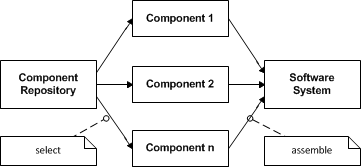
\includegraphics[scale=0.75]{plug-in/component-based.png}
  \caption{Component-based software development \cite{Pour} }
  \label{fig_cbsd}
\end{figure}

Other benefits that Component-based software development brings and we believe U-Sem will benefit from include: significant reduction of development cost and time-to-market, and also improvement on maintainability, reliability and overall qualities of software systems \cite{Pour1} \cite{Pour2}. Additionally, the applicability of this this approach is supported by the fact that is widely used in both the research community and in the software industry. There are many examples of technologies implementing this approach including: OMG's CORBA,  Microsoft's Component Object Model(COM) and Distributed COM (DCOM), Sun's(now Oracle) JavaBeans and Enterprise JavaBeans, OSGI.

\subsection{Component model}

Designing the component model of a system provides the specification defining the way that the system can be build by composing different components applying the component-based software engineering approach. More formally, it is the architecture of a system or part of a system that is built by combining different components \cite{Cai}. It defines a set of  standards for component implementation, documentation and deployment. Usually, the main components that a component-based software system consists of are \cite{Chen}:

\paragraph{Interfaces}
	determine the external behaviour and features of the components and allow the components to be used as a black box. They provide the contract which defines the means of communication between components. As illustrated on figure \ref{fig_intf}, interfaces can be considered as points where custom functionality provided by another component can be plugged in. 
	
	\begin{figure}[h!]
  		\centering
  		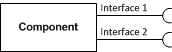
\includegraphics[scale=0.75]{plug-in/component-interfaces.png}
  		\caption{Component interfaces }
  		\label{fig_intf}
	\end{figure}

\paragraph{Components}
	are functional units providing functionality by implementing interfaces. As can be seen on figure \ref{fig_comp} components provide  features by implementing the interfaces provided by other components. One of the main question regarding building components is how to define the scope and characteristics for a component. According to \cite{Cai} there are no clear and well established standards or guidelines that define this. In general, however, a component has three main features: 

\begin{itemize}
	\item a component is an independent and replaceable part of a system that fulfils a clear function
	\item a component works in the context of a well-defined architecture
	\item a component communicates with other components by its interfaces 
\end{itemize}

	\begin{figure}[h!]
  		\centering
  		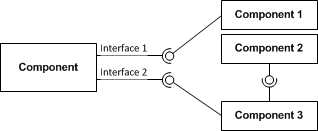
\includegraphics[scale=0.75]{plug-in/component-services.png}
  		\caption{Components implementing interfaces }
  		\label{fig_comp}
	\end{figure}

\paragraph{Coordinator}
	is the entity which is responsible to glue together and manage all the components. It is needed because components provide a number of features, but they are not able to activate the functionality themselves. This is the responsibility of the coordinator.

\subsection{State of the art component model implementations}

In previous sections discussed that integrating a component model in the architecture of U-Sem is the scientifically proven approach that promises to solve the design problem and fulfil the requirements of the customers. However, before designing and implementing our own component model, we continued with the scientific research to discover if there are already existing technologies that can be reused. Reusing a popular and widely used solution might be beneficial because it is likely it is heavily tested(at least from the engineers using it) and thus provide higher quality. 

\cite{Lau} suggests classification of the component model implementations based on which part of the life cycle of a system the composition of the components is done. They identify the following groups:

\begin{itemize}
	\item  Composition happens during the design phase of the system. Components are designed and implemented in the source code of the system.
	\item  Composition happens during the deployment phase. Components are constructed separately and are deployed together into the target execution environment in order to form the system.
	\item Composition happens during the runtime phase. Components are put together and executed in the running system.
\end{itemize}

For the architecture of U-Sem we are only interested in the last group since one of the main requirements is that scientists should be able to add, update and remove components while the system is running, without restarting it. It is essential since the system is used by multiple scientists and any system restart will cause temporary unavailability of all services. 

Apart form this, there is also another critical concern when choosing component model implementation for U-Sem. The implementation should support the Java language since it is the language in which all current services are implemented and most scientists are familiar with. Having to learn a new language and/or rewriting all source code in different language is considered as a big disadvantage for the scientists.

We performed an investigation in order to find what are the current state of the art technologies that satisfy all requirements. It showed that currently there two standards that satisfy our needs: Fractal \cite{Bruneton} and Open Services Gateway initiative (OSGI) \cite{OSGI}. Both of them seemed quite popular and widely used and therefore we concluded that reusing them is more beneficial than implementing a component model from scratch. For the proposed architecture of U-Sem we chose to use OSGI since our impression is that it provides a simpler way of defining components(no component hierarchies) which will be beneficial for scientists that do not have so in depth knowledge of component-based engineering. OSGI is also widely used\cite{Andre} which may suggest that it is well tested and therefore is more stable. Next subsection focuses on how OSGI works and its features that are interesting for the architecture of U-Sem.


\subsection{OSGI}

Proposed first in 1998, OSGI represents a set of specifications that defines a component model which represents a dynamic component system for Java. These specifications enable a development model where applications are dynamically composed of different independent components. Components can be loaded, updated and deleted on demand without having to restart the system. OSGI implements the main components of the standard component model which are discussed in the previous section as follows:

\begin{figure}[h!]
  \centering
  	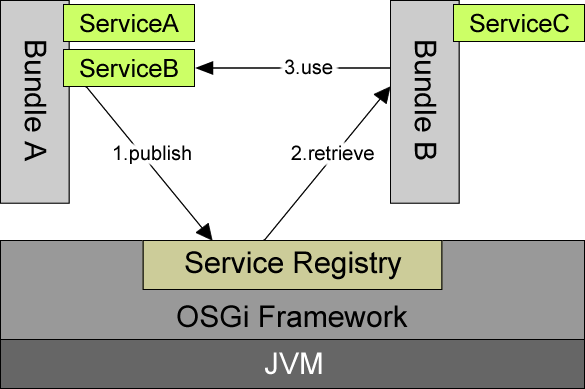
\includegraphics[scale=0.6]{plug-in/OSGI.png}
  \caption{OSGi Service Registry \cite{Andre}}
  \label{fig_osgi}
\end{figure}

\paragraph{Interfaces}
 in OSGI define the contract for communication between different components by describing the operations that has to be implemented by the components. Basically, they represent standard Java interfaces which has to be available to both the component that implements the interface and the components that use the implemented functionality.


\paragraph{Components}
  in OSGI are called bundles. Bundles are basically a regular Java JAR files that contain class files and other resources such as images, icons, required libraries. One of the important benefits for U-Sem is that OSGI enables better modularization providing facilities for better information hiding then the one provided by the Java language \cite{Andre}. Each bundle should provide a manifest file, which enables engineers to declare static information about the packages that are exported and therefore can be used by other bundles. Furthermore, bundles provide functionality to the rest of the system in the form of services. In the OSGi architecture, services are standard Java objects that implement the interfaces described in the previous paragraph.

\paragraph{Coordinator}
The OSGi standard also provides coordinator component which represents a runtime infrastructure for controlling the life cycle of the bundles which includes adding, removing and replacing bundles at run-time, while preserving the relations and dependencies among them. Another key functionality that the coordinator component of OSGi provides is the management of the services provided by the bundles. This functionality is provided by the Service Registry, which keeps track of the services registered within the framework. As illustrated on Figure \ref{fig_osgi} when a bundle is loaded it registers all the services that it implements(step 1). As soon as a service is registered it can be retrieved by any other components that are interested in this functionality (step 2). Once a bundle has retrieved a service, it can invoke any method described by the interface of this service (step 3). Another interesting feature of the OSGi Service Registry is its dynamic nature. As soon as a one bundle publishes a service that another bundle is interested in, the registry will bind these two bundles. This feature is very important for U-Sem since it will enable scientists to plug in any new functionality dynamically when it is needed.


\section{Architecture}
\label{sec:architecture}

This section describes the architecture of U-Sem regarding the dynamic component model. In order to provide more efficient description we have provided a set of interrelated views, which collectively illustrate the functional and non-functional features of the system from different perspectives and demonstrate that it meets the requirements.

\subsection{Context View}

This section discusses the runtime environment of U-Sem. As explained in the introduction section initially the system only communicated with providers of semantic content and the clients which execute the services. However, introducing the dynamic component model of U-Sem we bring to entities on the stage. Figure \ref{fig_context} illustrates the updated runtime environment of U-Sem.

\paragraph{Scientists}
As one can see on the diagram the system also communicates with the scientists in order to enable them to plug-in new functionality. When scientists want to add new functionality they first have to build a component that encapsulates the new logic. Then they upload the component to U-Sem and it will be installed in the components space of the scientist. Once installed, the scientist can start using the newly added functionality. Scientists can also communicate with U-Sem in order to manage the existing components loaded into the system. They can view the list of all available components and if needed they can also update or even remove them. 

\begin{figure}[h!]
  \centering
  	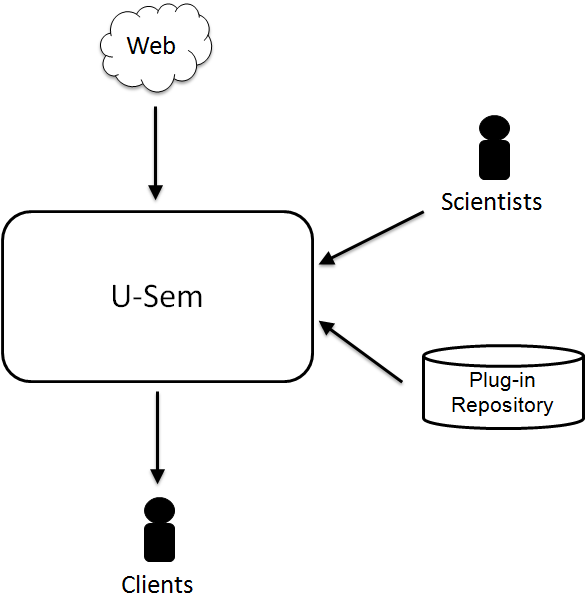
\includegraphics[scale=0.5]{plug-in/environment/runtime_env.png}
  \caption{Context diagram of U-Sem }
  \label{fig_context}
\end{figure}

\paragraph{Plug-in repository}
Another interesting addition to the environment is the Plug-in repository. It represents a storage location where plug-ins are stored and when needed, they can be retrieved and installed into the system. Scientists build and then publish their plug-ins there so that anyone interested can install and use them. The need for this approach emerges from the fact that scientists has to be able to share their components with one another.

By using the Plug-in repository scientists are able to share components before they are installed into U-Sem. Alternative approach would have been enable scientists to share already installed components between each other. In this way whenever a scientist creates a new version or entirely new component it is installed to U-Sem, shared and then all other scientists are able to use it. However, this approach has one major disadvantage. When a new version of a component is installed then all scientists automatically start to use the new version. The version, though, might introduce a bug or it might not be completely compatible with the previous version. As a result, all other scientists' services and components that are using it are threatened to experience failures. 

Using the Plug-in repository overcomes this problem. When a scientist releases new version of component, other scientists can decide whether or not to immediately adopt the new release. If they decide not to, they can simply continue using the old one. Otherwise, when they decide that are ready for the change, they install and use the new release. The benefit from this is that none of the scientists are at the mercy of the others. Changes made to one component do not need to have an immediate affect on other scientists that are using it. Each scientist can decide weather or when to move to the new releases of the components in use. This approach is already adopted in the industry \textbf{TODO P2, Eclipse etc.}


\subsection{Process modelling}

Once we have already identified the new actors(scientists) and external systems(plug-in repository) in the runtime environment of U-Sem we have to define how they interact between each other. In this section we will use the Business Process Management Notation(BPMN) \cite{BPMN} to model the business processes that defines the interactions needed in each of the use cases that regard the dynamic component model feature of U-Sem. It also enables to model activities, decision responsibilities, control and data flows. The decision to use BPMN to model the interactions is based on its relative suitability for interaction modelling and the fact that it is more popular compared to its alternatives \cite{Decker}. Next subsections describe each of the defined processes and expand them into Business Process Diagrams (BPD).

\subsubsection{Create U-Sem Component process}

Creating new functionality for U-Sem is the most important use case regarding the dynamic component model feature. We modelled this use case as the \textit{Loading new components} business process. Figure \ref{fig_install_bpm} provides the business process model diagram that illustrates this process. 

As illustrated in the diagram there are three participants in this process(U-Sem, Scientists and Plug-in repository) which are illustrated in separate BPMN pools. When a scientist wants to create new functionality for U-Sem, he/she firsts writes the source code, providing all required resources and implementing the desired U-Sem interfaces(the component interfaces discussed in previous sections). Then everything has to be build and encapsulated into a component. Once the component is ready, scientists can directly upload it to U-Sem if the component is only for private use. When U-Sem receives a component it is responsible to installed it into the scientist's component storage please and make available all functionality provided by the component. Finally, U-Sem sends confirmation message back to the scientist. Alternatively the scientist might also want to share the component with other scientists. In this case the component is sent to the plug-in repository. When received, the repository is responsible to store it and make it available to the other scientists. Again at the end confirmation message is send to the scientist.

\begin{figure}[h!]
  \centering
  	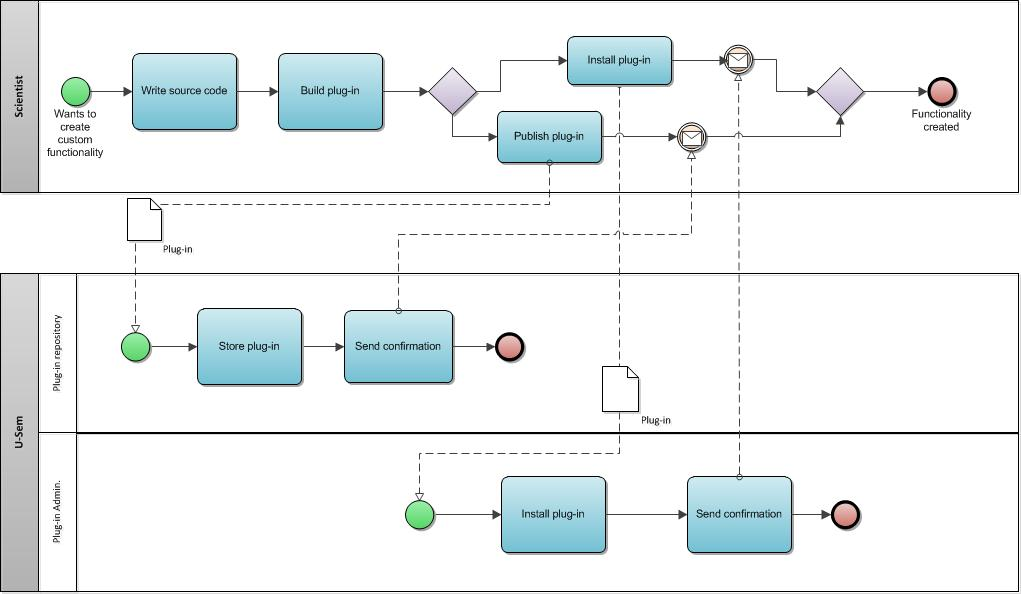
\includegraphics[scale=0.7,angle=90]{plug-in/business_processes/CreatePlugInBusinessModel.jpg}
  \caption{Business model describing the process for adding new plug-in to U-Sem}
  \label{fig_install_bpm}
\end{figure}

\subsubsection{Reuse shared components}

As already explained, U-Sem also enables scientists to reuse components shared by other scientist. This use case is modelled into the \textit{Reuse shared components} business process which is illustrated in Figure \ref{fig_repo_bpm}. Again we have three participants in this process(U-Sem, Scientists and Plug-in repository) which are illustrated in separate BPMN pools. 

The process consists of two main phases. First, the scientist contacts the plug-in repository in order to determine what are the currently available components. Secondly, he/she contacts U-Sem providing information about the desired component/s. U-Sem then contacts the plug-in repository in order to get the components. Finally, the provided components are stored into the private space of the scientist and a confirmation message is send back.

\begin{figure}[h!]
  \centering
  	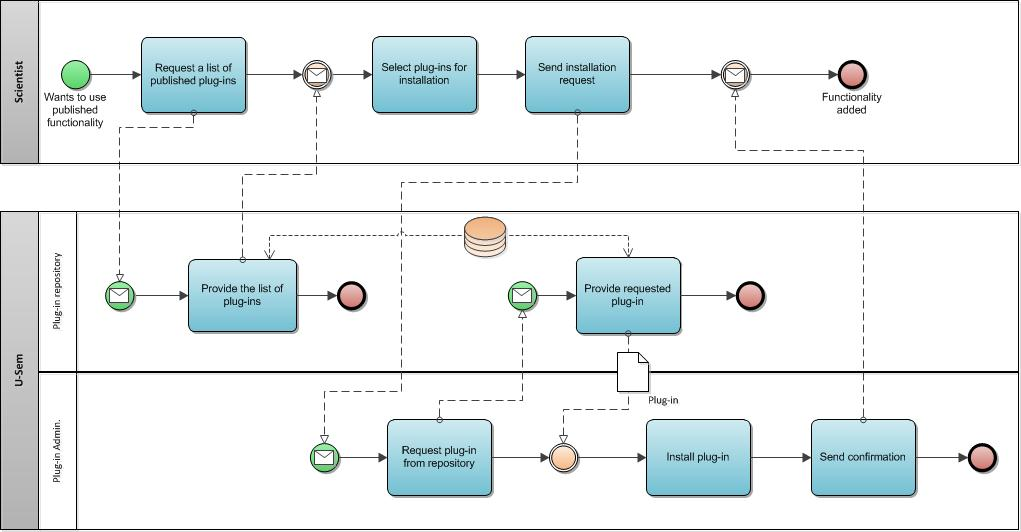
\includegraphics[scale=0.7,angle=90]{plug-in/business_processes/InstallPlugInFromRepoBusinessModel.jpg}
  \caption{Business model describing the process for adding existing plug-in from repository to U-Sem}
  \label{fig_repo_bpm}
\end{figure}

\subsubsection{Component Management}

Managing components is also another important use case. Implementing it will enable scientists to view all components installed into U-Sem and if needed remove them. This use case was modelled into the \textit{Component Management process} which is illustrated on Fugure \ref{fig_admin_bpm}. In this case we have interaction only between the scientist and U-Sem.

Scientists can monitor the currently installed components at any time by contacting U-Sem. When such request is received, U-Sem is responsible to send back detailed information about all the components. Having this lists, scientist are also able to remove components. In this case scientists have to submit request for removal providing detailed for the component that has to be removed. Upon receiving such request U-Sem is responsible to permanently remove the component form the private space of the scientists and when finished send back a confirmation message.

\begin{figure}[h!]
  \centering
  	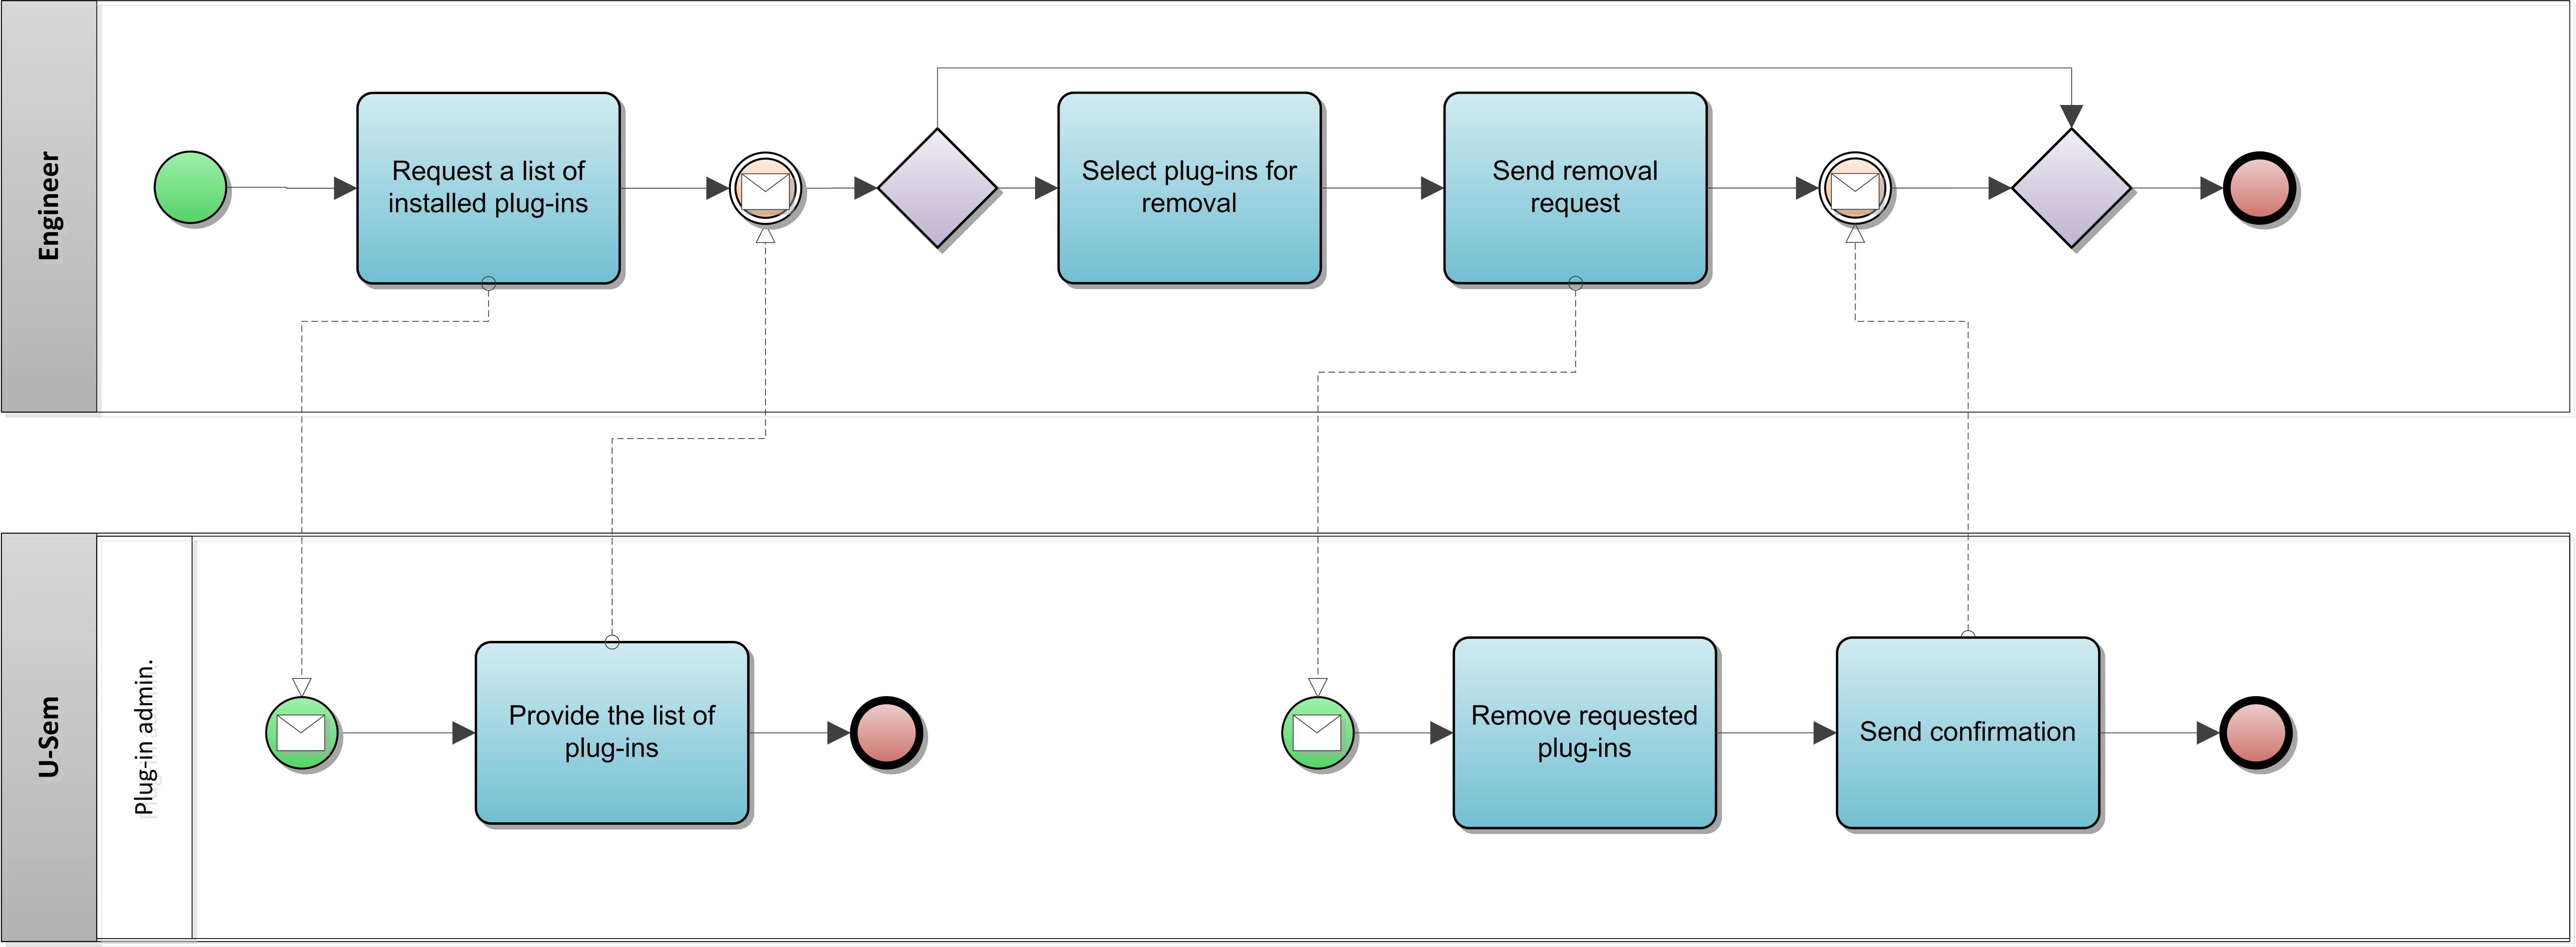
\includegraphics[scale=0.6]{plug-in/business_processes/PluginManagementBusinessModel.jpg}
  \caption{Business model describing the process for managing plug-ins in U-Sem}
  \label{fig_admin_bpm}
\end{figure}


\subsection{Functional view}

After identifying all actors that that are part of the environment of U-Sem and the way they interact with one another, it is now time to discuss the internal structure of U-Sem that accommodates all these interactions. This section defines the architectural elements that provide the functionality of the system. It describes the functional structure of the system including the key functional elements, their responsibilities, the interfaces they expose, and the interactions between them. Taken together, this demonstrates how the system will perform the required functions.

All components that are take part in the dynamic component model functionality can be classified in layers. This three layered organization is illustrated in figure Figure \ref{fig_layer} and defines the following layers:

\begin{figure}[h!]
  \centering
  	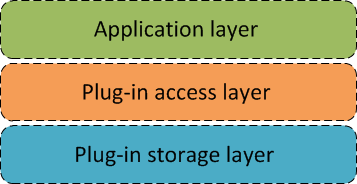
\includegraphics[scale=0.6]{plug-in/layers/layers.png}
  \caption{Layer organization of U-Sem}
  \label{fig_layer}
\end{figure}

\begin{itemize}
	\item \textit{Plug-in storage layer} is responsible to provide storage functionality for storing the installed plug-ins. Additionally, it should provide place where plug-ins can store data during their execution.
	\item \textit{Plug-in access layer} provides functionality for plug-in management and provides access to services provided by the components. Components in this layer are responsible to enforce the security, privacy, etc. policies of the system.
	\item \textit{Application layer} this layer consists of all components that are interested in using the services provided by the plug-ins. These applications are also responsible to provide functionality to the user for adding new plug-ins to the system or managing the existing once. 
	\end{itemize}

\subsubsection{High-level organization}

This section describes the internal structure of the layers and specifies the high level components that build up the feature. Figure \ref{fig_comp} illustrates this organization and shows how the high-level components are organized into the layers. We have the following components starting from bottom up:\textbf{TODO better explanation is needed}

\begin{figure}[h!]
  \centering
  	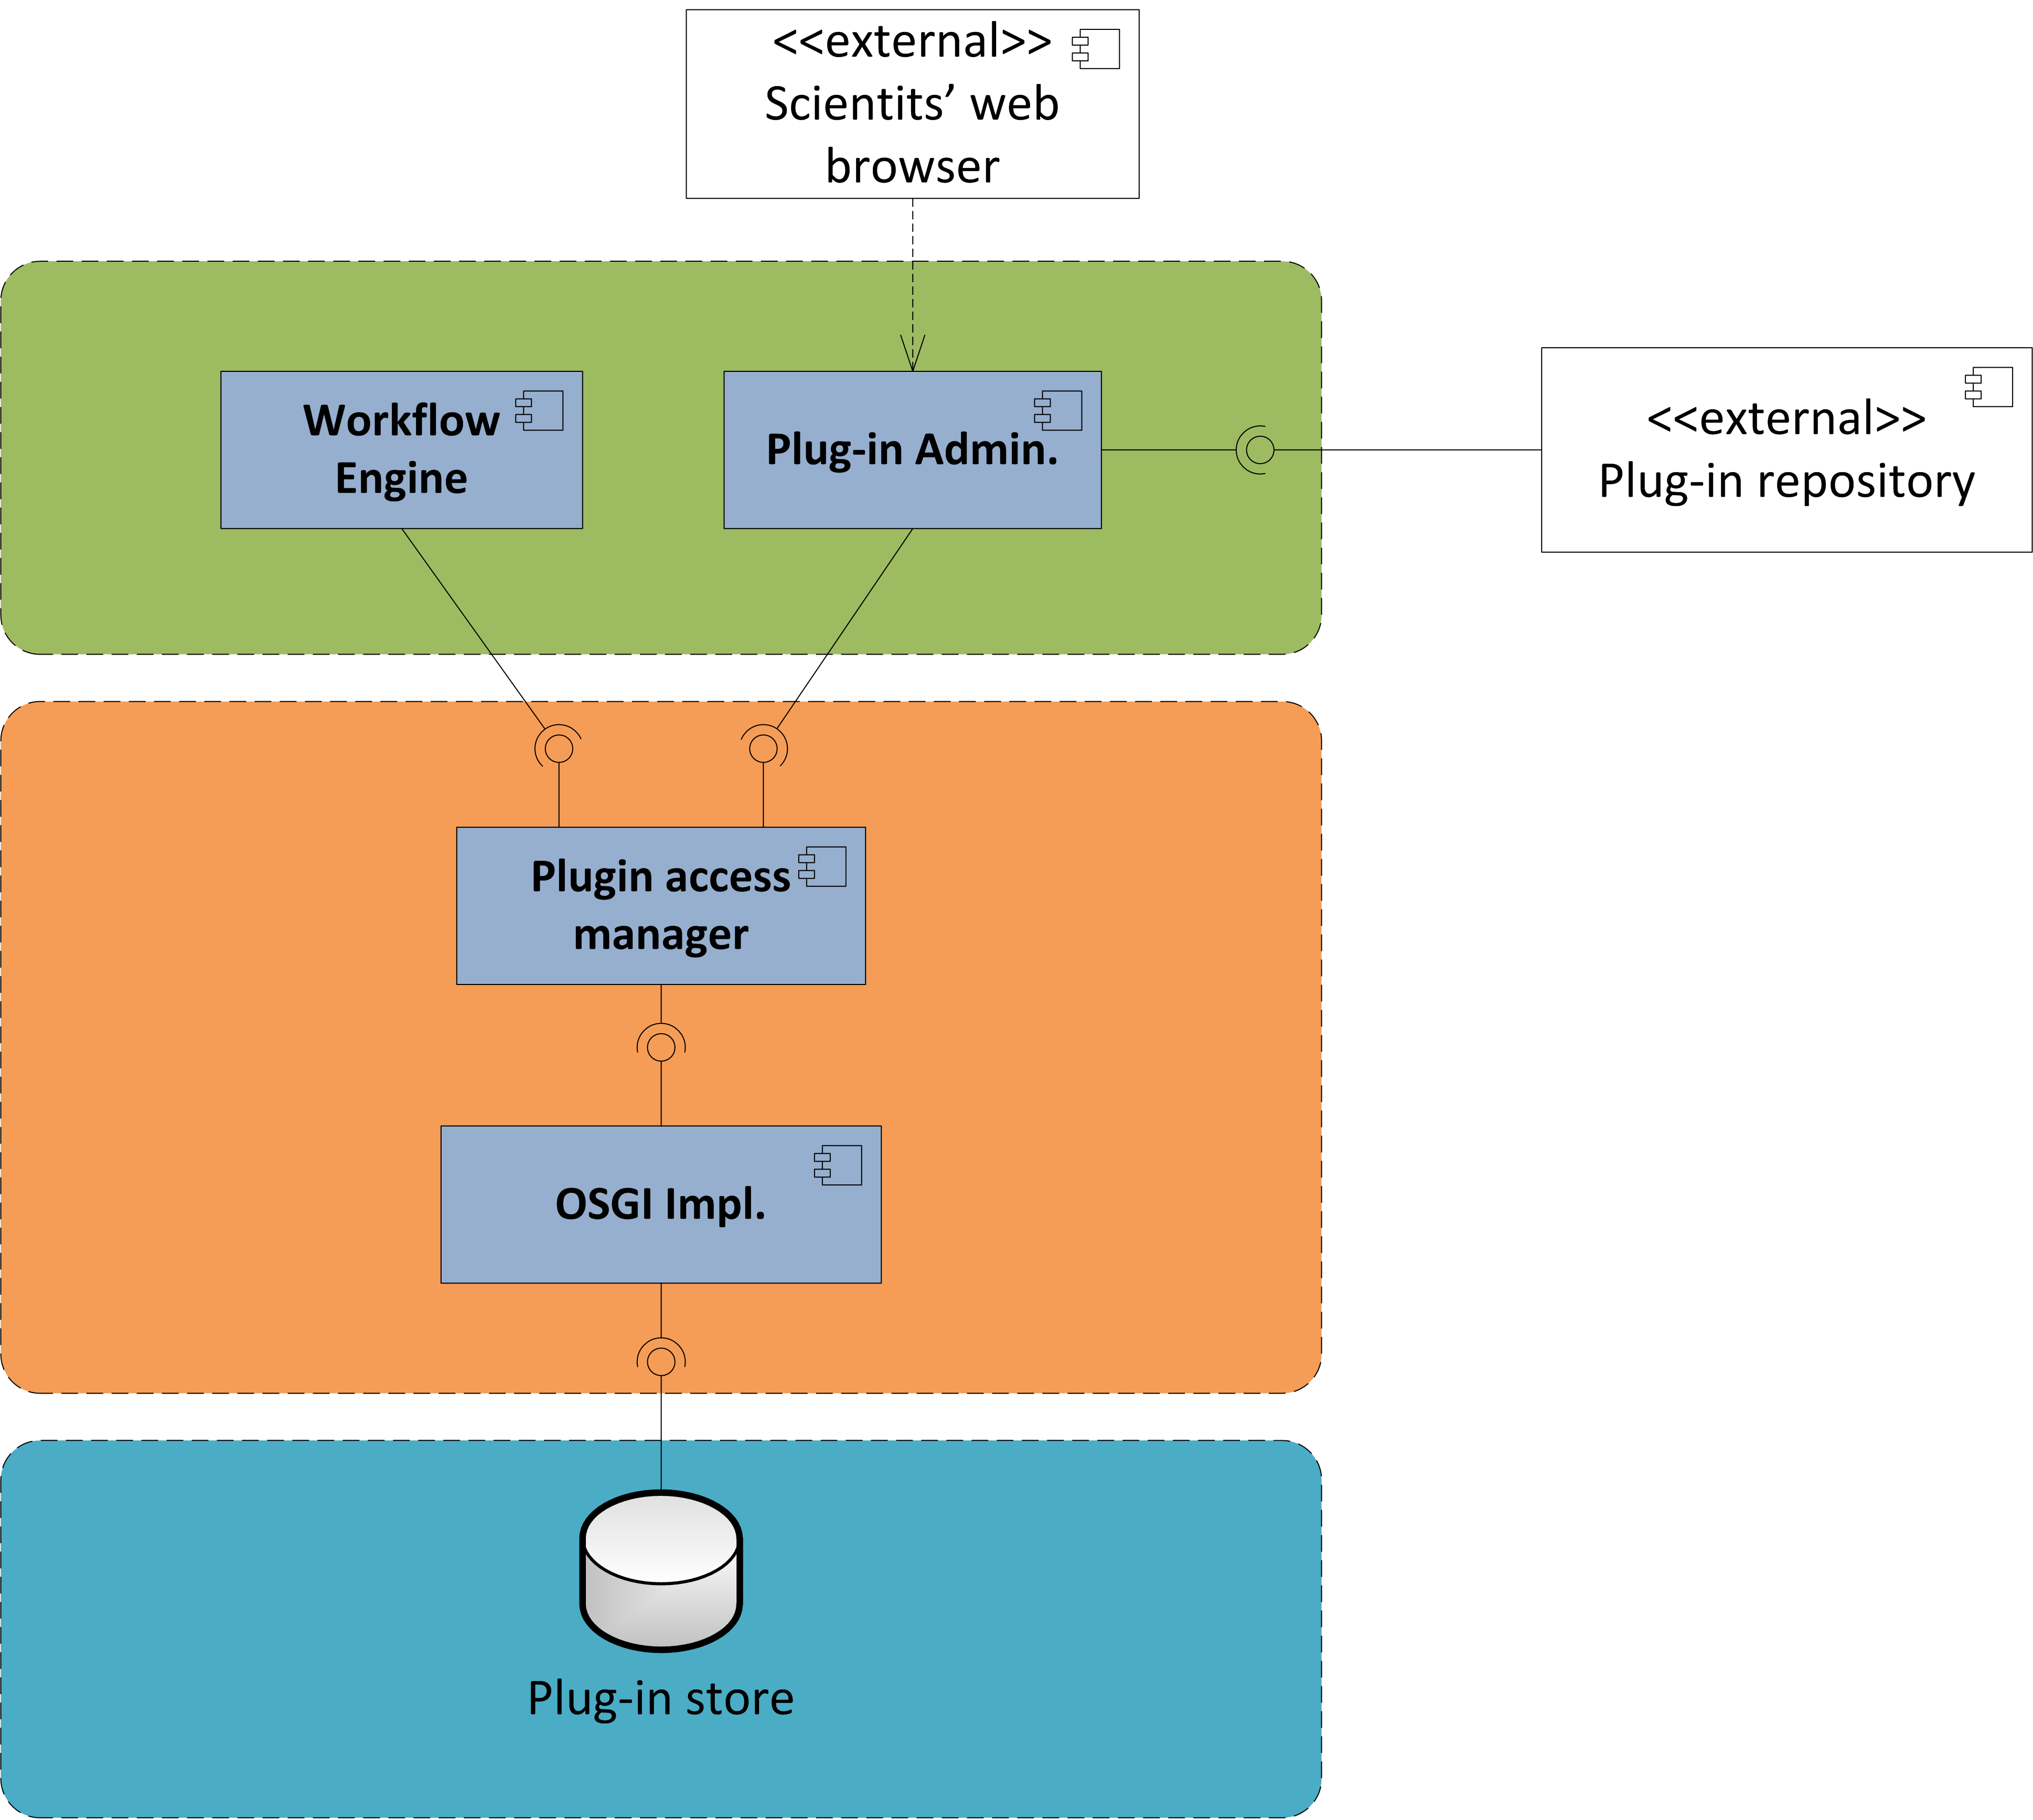
\includegraphics[scale=0.6]{plug-in/layers/main-func.png}
  \caption{Component diagram illustrating the functional organization of U-Sem}
  \label{fig_comp}
\end{figure}

\begin{itemize}

\item \textit{Plug-in Store} is responsible to store the installed plug-ins for each user. It should provide permanent store for the components so that after system restart they are still available. This component is also responsible to provide storage space for each component in case any data storage is required. Current implementation of OSGI can only operate with file store and therefore this component is represented by the file system of the operating system. For availability reasons this storage should be \textbf{replicated}.

\item \textit{OSGI Implementation} - As we already discussed in previous sections, we chose OSGI as a standard for achieving the dynamic component model for U-Sem. It is responsible to keep track of plug-ins life cycle(create, store, ..) and provide access to the services implemented by the different components. It provides API which enables communication with the framework.

\item \textit{Plug-in access manager} acts as a level of abstraction over the OSGI component. It is responsible to deal with the configuration ans start of the framework. It is also responsible to enforce the security policy and provide insulation between scientists. It provides API for the higher level components for dealing with services and management of plug-ins. Further decomposition of this component is provided in the next section.

\item \textit{Plug-in admin.} is responsible to deal with the administration of the plug-ins. It provides the system's endpoint(UI) for interaction with the scientist scientists. Further decomposition of this component is provided in the next section. 

\item \textit{Workflow engine} uses the interface provided by the \textit{Plugin access manager} to get list of the available services and when required execute them.
	
\end{itemize}


\subsubsection{Plug-in admin. module}

This section defines the functional decomposition of the Plug-in admin. module which is illustrated in figure \ref{fig_admin_func}. It consists of the following components:

\begin{figure}[h!]
  \centering
  	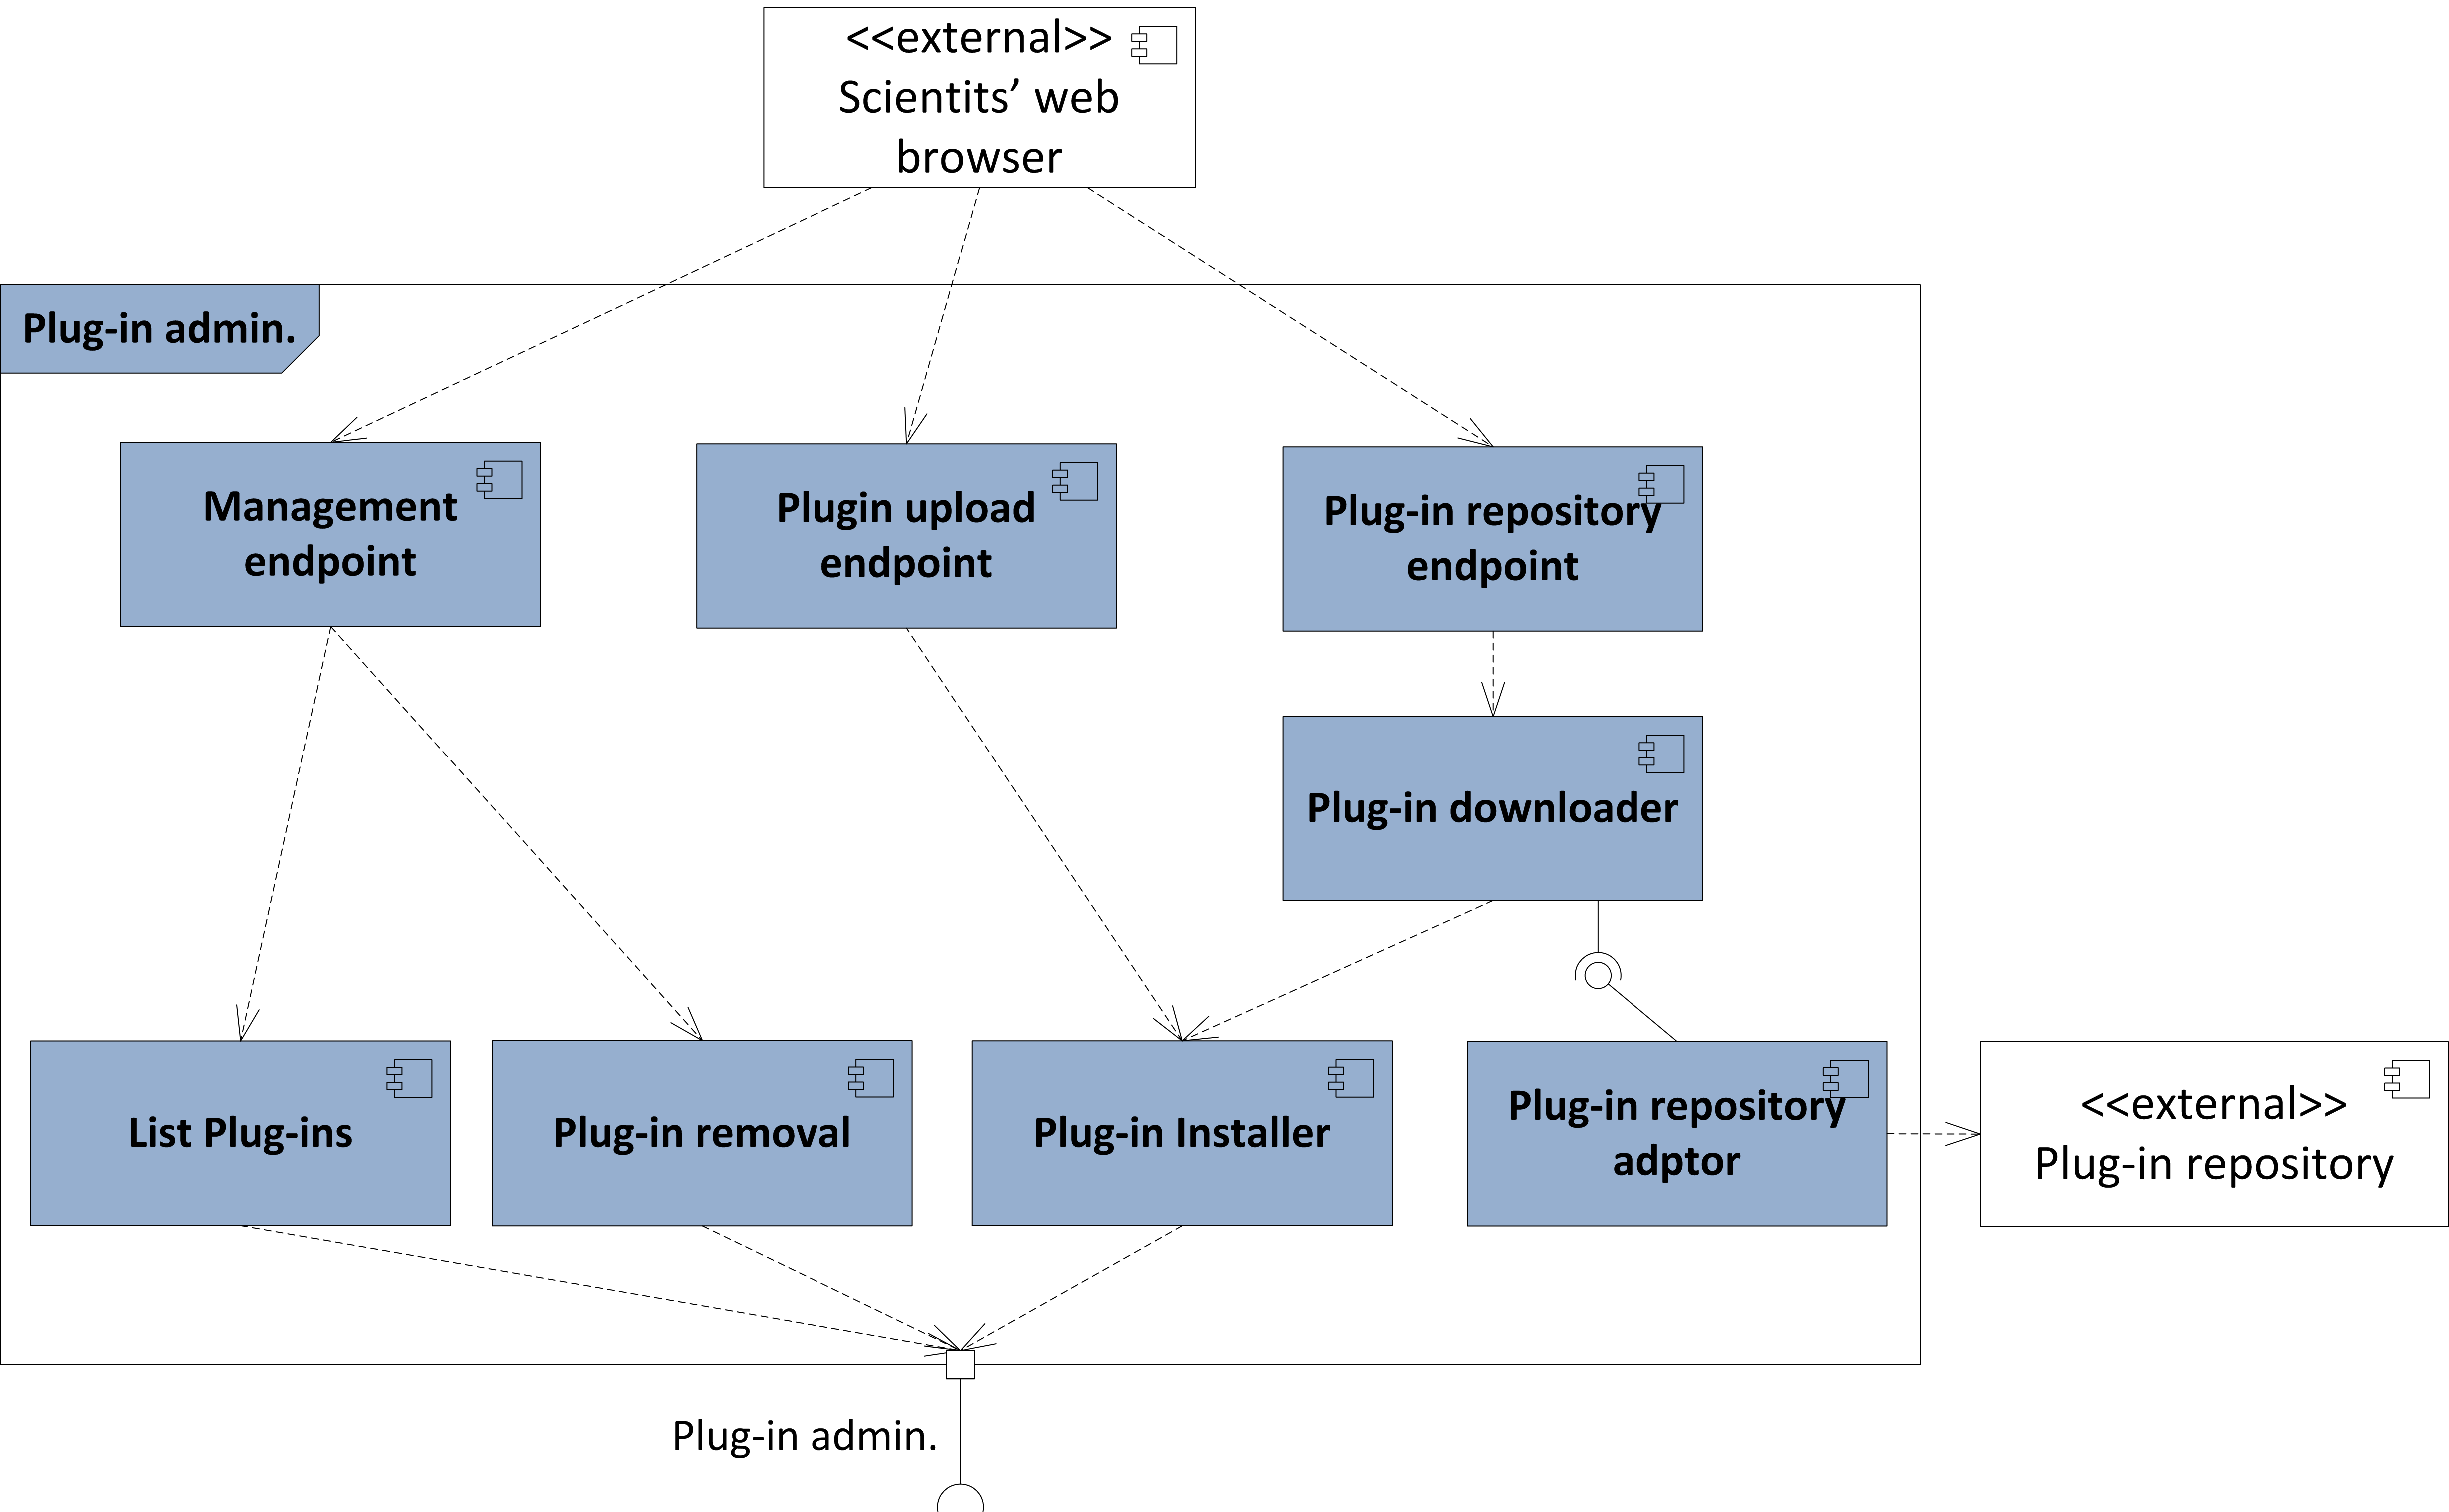
\includegraphics[scale=0.75]{plug-in/layers/admin-func.png}
  \caption{Functional decomposition of the \textit{Plug-in admin.} module}
  \label{fig_admin_func}
\end{figure}

\begin{itemize}

\item \textit{List Plug-ins} - This component is responsible to provide functionality that provides the list of all plug-ins that are installed for the particular user. This component has to provide detailed information for each plug-in: its id, name, vendor, etc.

\item \textit{Plug-in removal} - This component should enable users to remove(uninstall) plug-ins.  

\item \textit{Management endpoint} - This component provides the user interface for the plug-in management functionality. It acts as a bridge between the user and the components that provide the actual functionality. 

\item \textit{Plug-in installer} - This component receives a plug-in in the form of a \textit{jar} file and is responsible to install it to the storage space of a particular user.

\item \textit{Plug-in upload endpoint} - This components provides the user interface needed for uploading plug-ins. It enables users to select a \textit{jar} file from their local file system and upload it for installation.

\item \textit{Plug-in repository adaptor} - This component manages  the communication with the plug-in repository. It acts as a level of abstraction. U-Sem has to be able to use different repositories and this component is the only component to change if support for a new repository system is needed. 

\item \textit{Plug-in downloader} - This component is responsible to download the desired plug-ins from the repository and upon successful download notify the \textit{Plug-in installer} to continue with the  installation of the plug-in.

\item \textit{Plug-in repository endpoint} - This component provides the user interface which enables users to browse the plug-in repository and indicate which plug-ins should be downloaded and installed on U-Sem.

\end{itemize}


\subsubsection{Plug-in access manager}

This component is responsible to provide endpoint for the administrators to manage the plug-ins. They can install and delete plug-ins. This component is responsible to store and manage the access to all plug-ins. Figure \ref{fig_access_func} shows the functional decomposition of the Plug-in access manager module. It consists of the following components:


\begin{figure}[h!]
  \centering
  	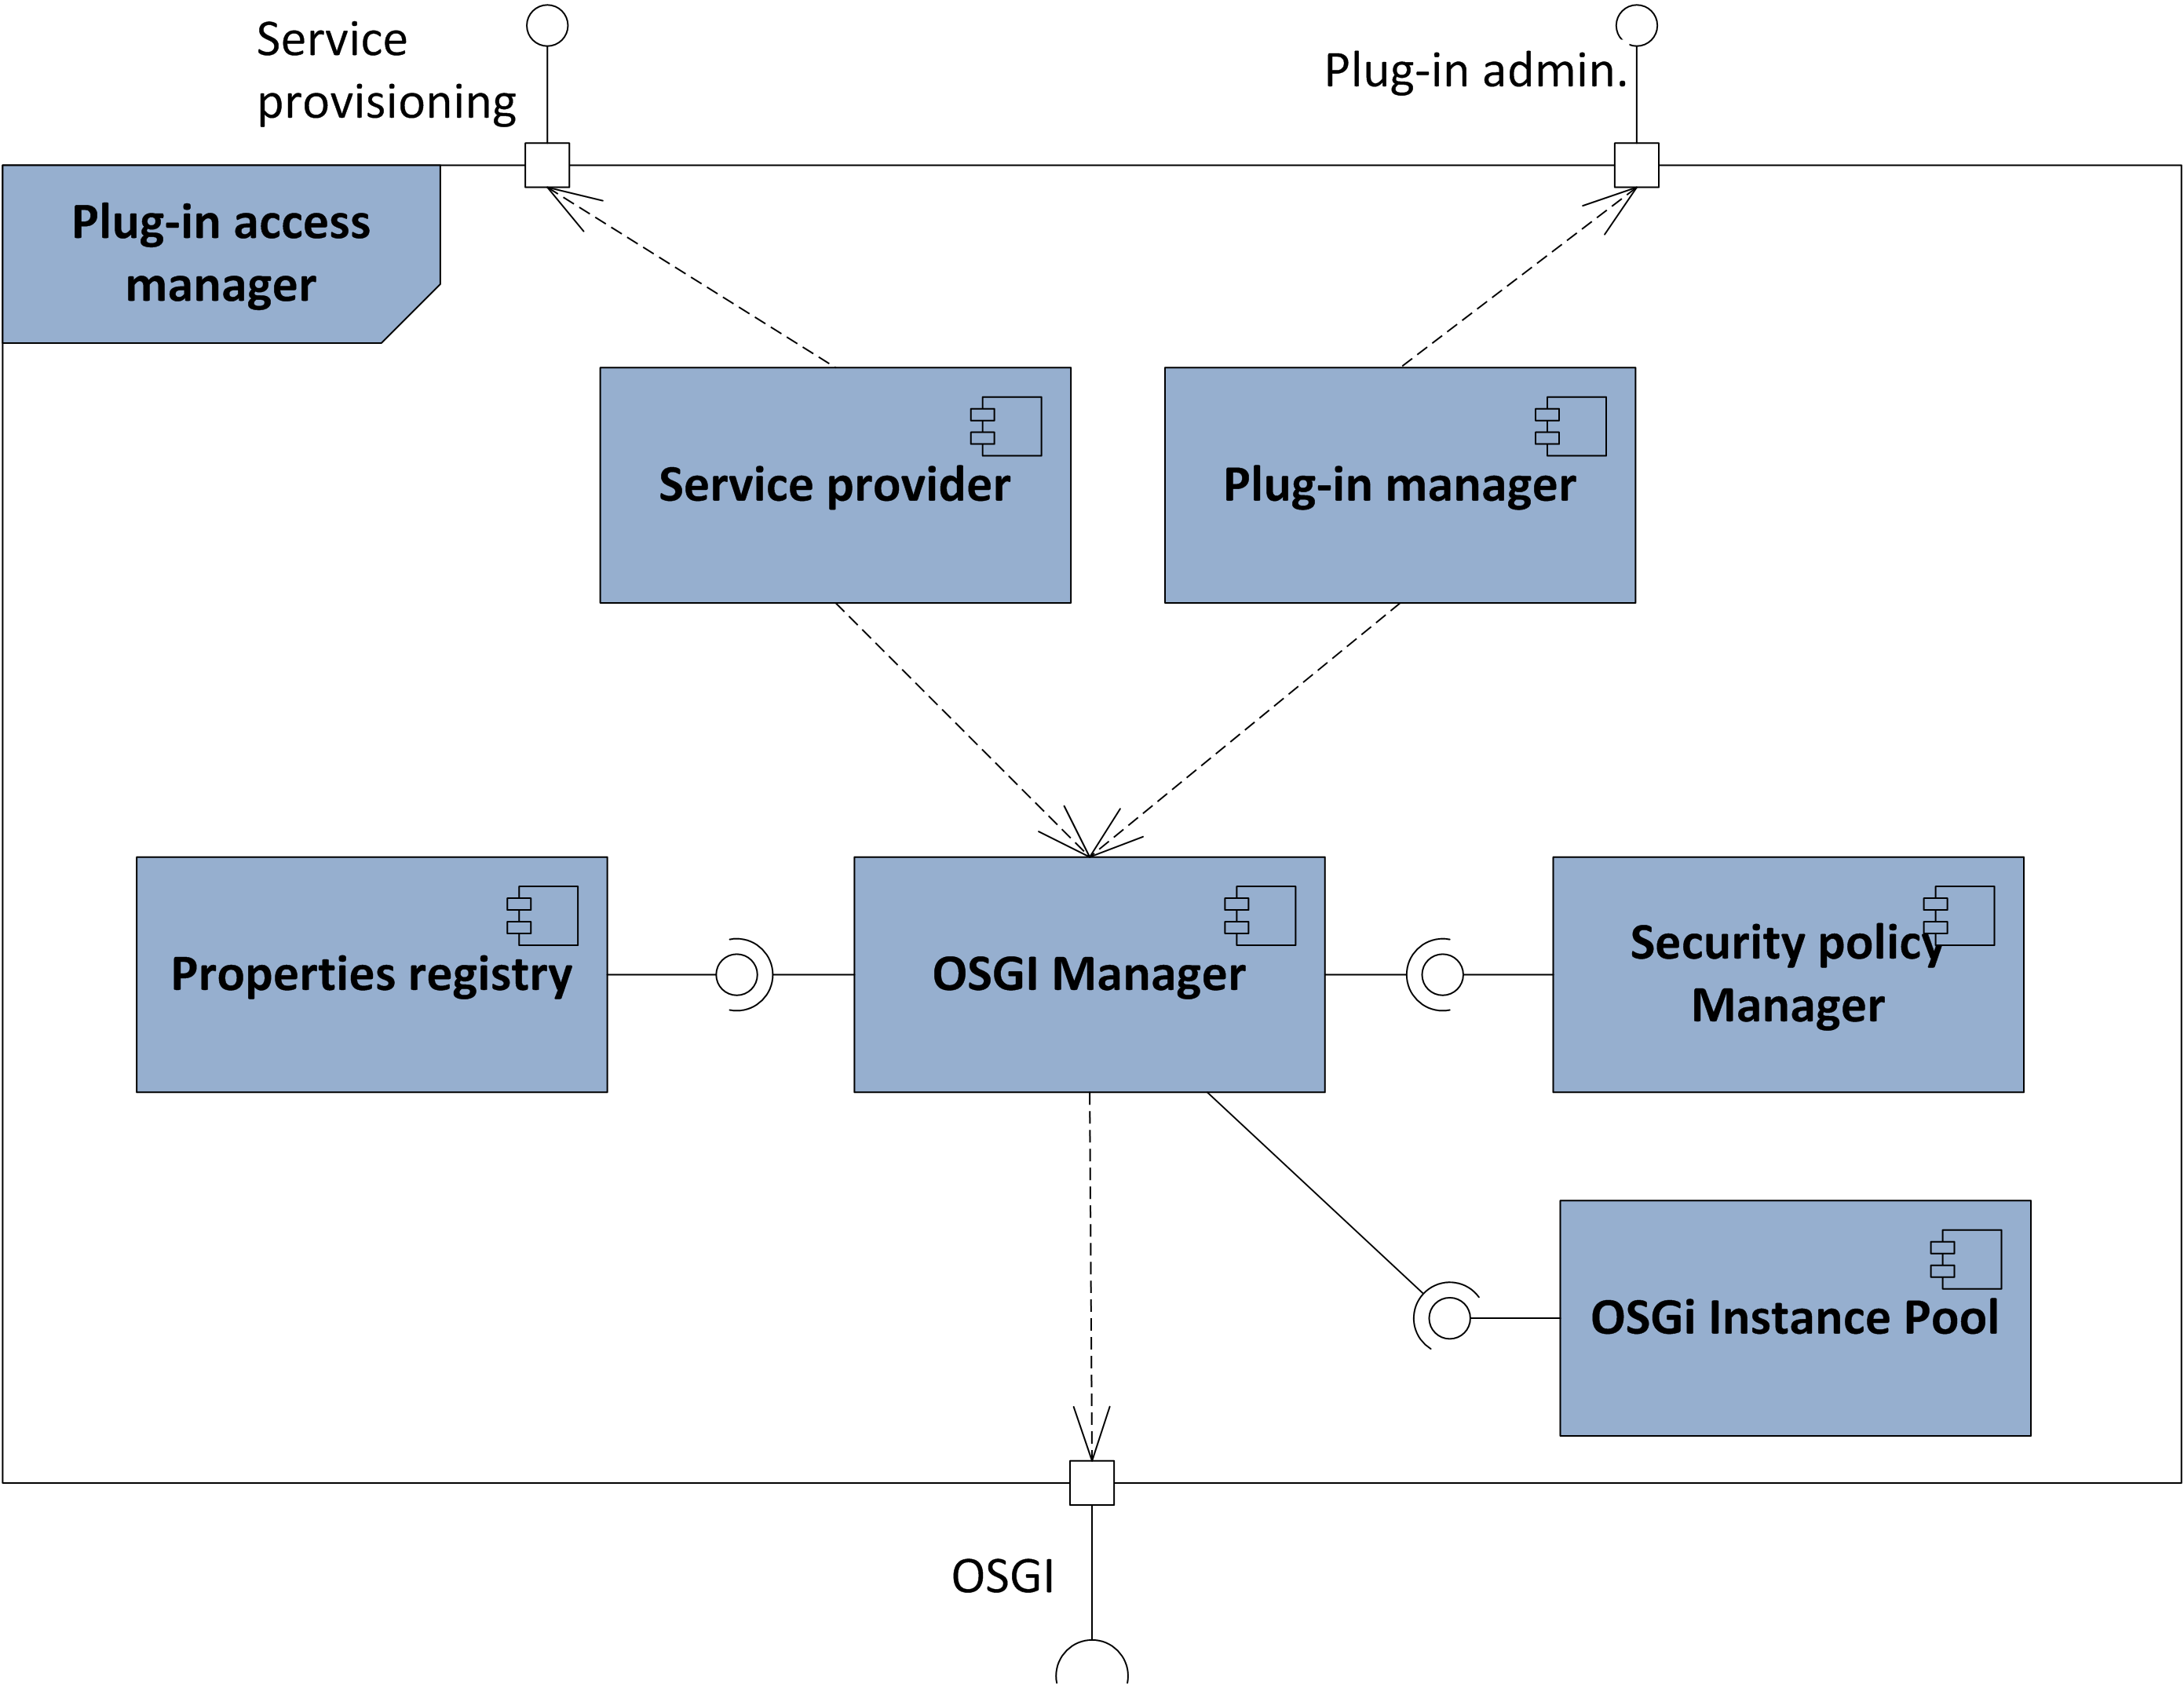
\includegraphics[scale=0.85]{plug-in/layers/access-func.png}
  \caption{Functional decomposition of the \textit{Plug-in access manager} component}
  \label{fig_access_func}
\end{figure}

\begin{itemize}

\item \textit{OSGI Manager} - This component manages the communication with the OSGI engine. It is responsible start/stop the engine and monitor its lifecycle. It is also responsible to enforce the security policies by setting up the Security Manager options of the engine. It also acts as a level of abstraction over the component engine and in case any change in future is required this is the only component that will be affected. 

\item \textit{Private space registry} - Keeps track for the storage space and settings for each user. It has to make sure that the storage places are not overlapping.  

\item \textit{Security policy} - Provides the security policy for each user. It defines the Java operations(file access \textbf{...}) that users are allowed to perform.

\item \textit{Plug-in manager} - This component is responsible to provide an API that is used by high level components to perform plug-in management tasks.

\item \textit{Service provider} - This component is responsible to provide an API that is used by high level components to get the list of available services and load them.

\end{itemize}

\paragraph{Security}

\subsection{Concurrency view}

This section describes the concurrency structure of U-Sem. We show how functional elements map to concurrency units(processes, process groups and threads) in order to clearly identify the parts of the system that can execute. We also show how this parallel execution is coordinated and controlled.

\begin{figure}[h!]
  \centering
  	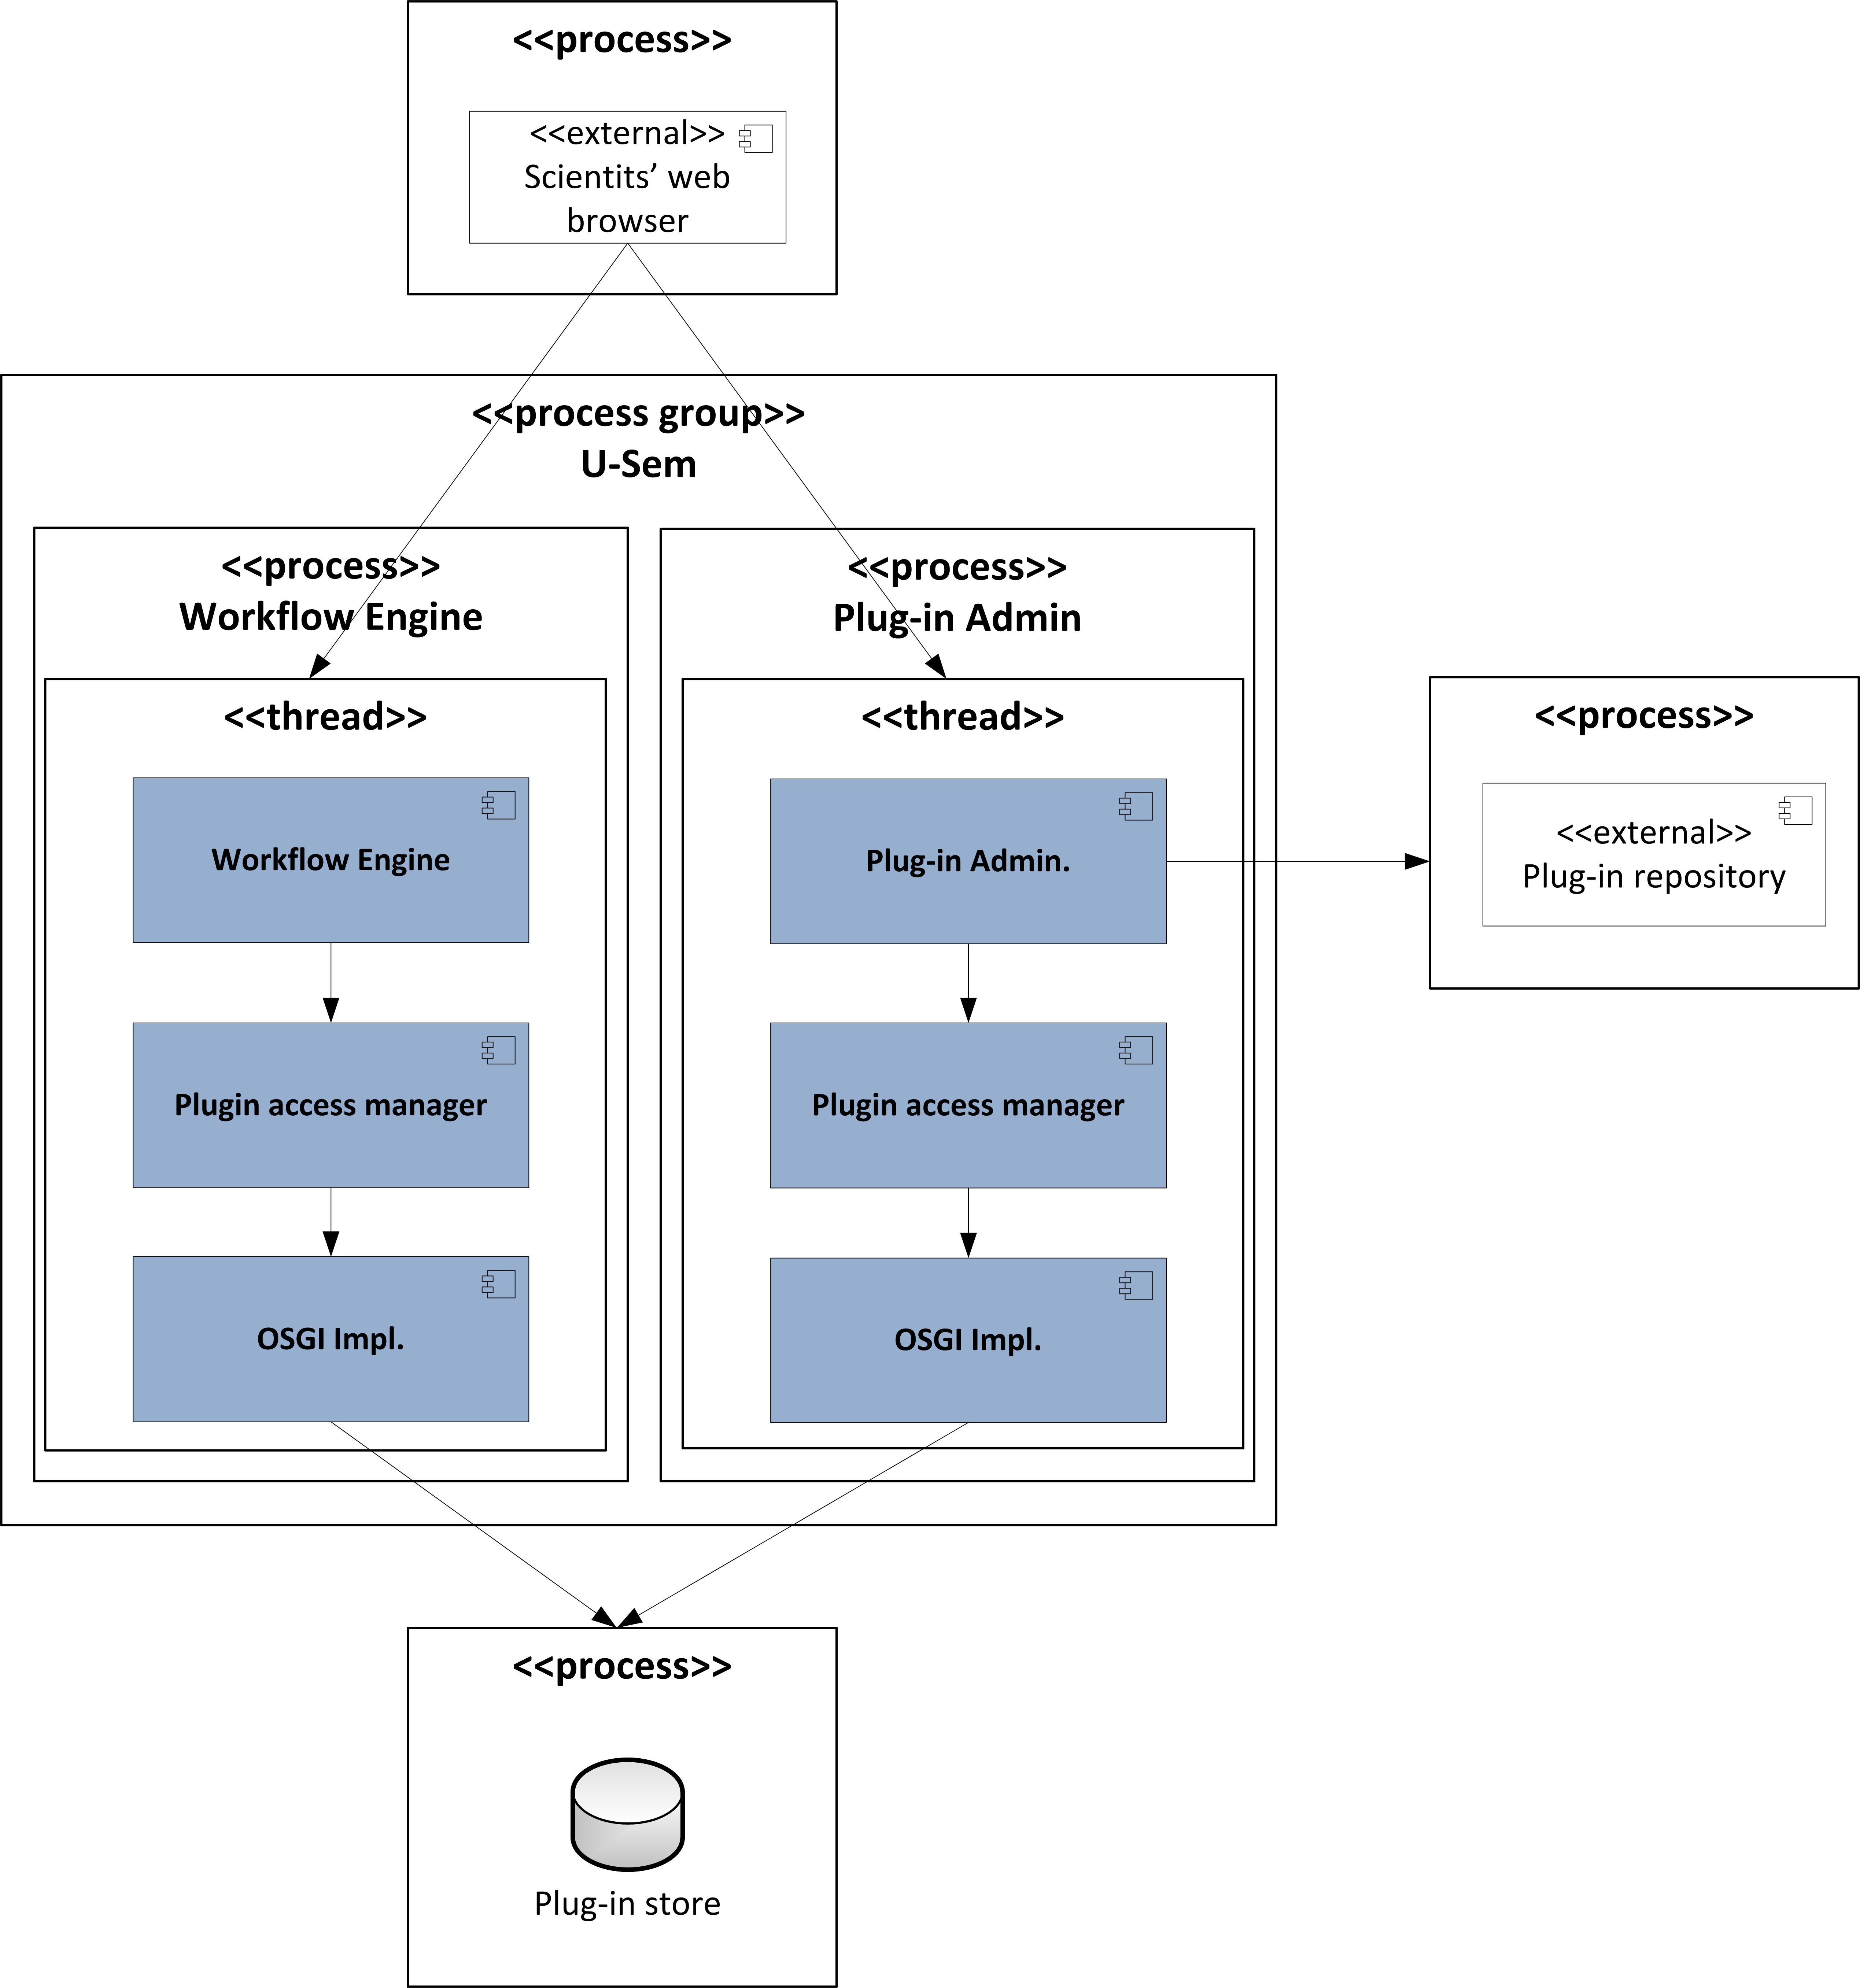
\includegraphics[scale=0.70]{plug-in/layers/concur.png}
  \caption{Diagram illustrating the concurrency model of U-Sem}
  \label{fig_conc}
\end{figure}

Figure \ref{fig_conc} illustrates the concurrency organization of U-Sem. The main functionality of the system is situated in the U-Sem process group. All U-Sem processes and all external processes(Plug-in repository) including the Database process operate concurrently. The main processes wait for requests from the user(web browsers and/or other systems). Each request is processed in separate thread depending on its type. As a result, multiple client requests can be handled simultaneously. Workflow execution initiated by U-Sem clients and plug-in manipulation by scientists can happen at the same time. However, the two processes does not communicate with each other and thus the synchronization on the installed plug-ins is achieved throw the storage process. Every time before executing a workflow, the process loads the isntalled plug-ins into the memory. This means any changes to the plug-ins during an execution of a workflow will not be applied and thus the execution will not be distrupted. All changes will take place the next time a workflow is executed.

\subsection{Deployment View}

This section describes the environment in which the system will be deployed. It defines where each of the processes defined in the previous section will run. 

Due to the nature in which the system operates we had to consider flexibility and scalability. In order to test their work scientists has to be able to easily install and set up U-Sem. In this scenario scalability and performance is not critical however simplicity is crucial. In production mode the system will be used by many users and many services will be running simultaneously. Therefore, in this situation the performance and scalability issues are most important. As a result, we designed U-Sem to be flexible and be able to accommodate both scenarios.



\subsubsection{Simple setup}

This setup targets the scenarios where there is no need for high performance and scalability. The aim is to enable scientists to  setup the system fast on a single machine and little configuration. 

\begin{figure}[h!]
  \centering
  	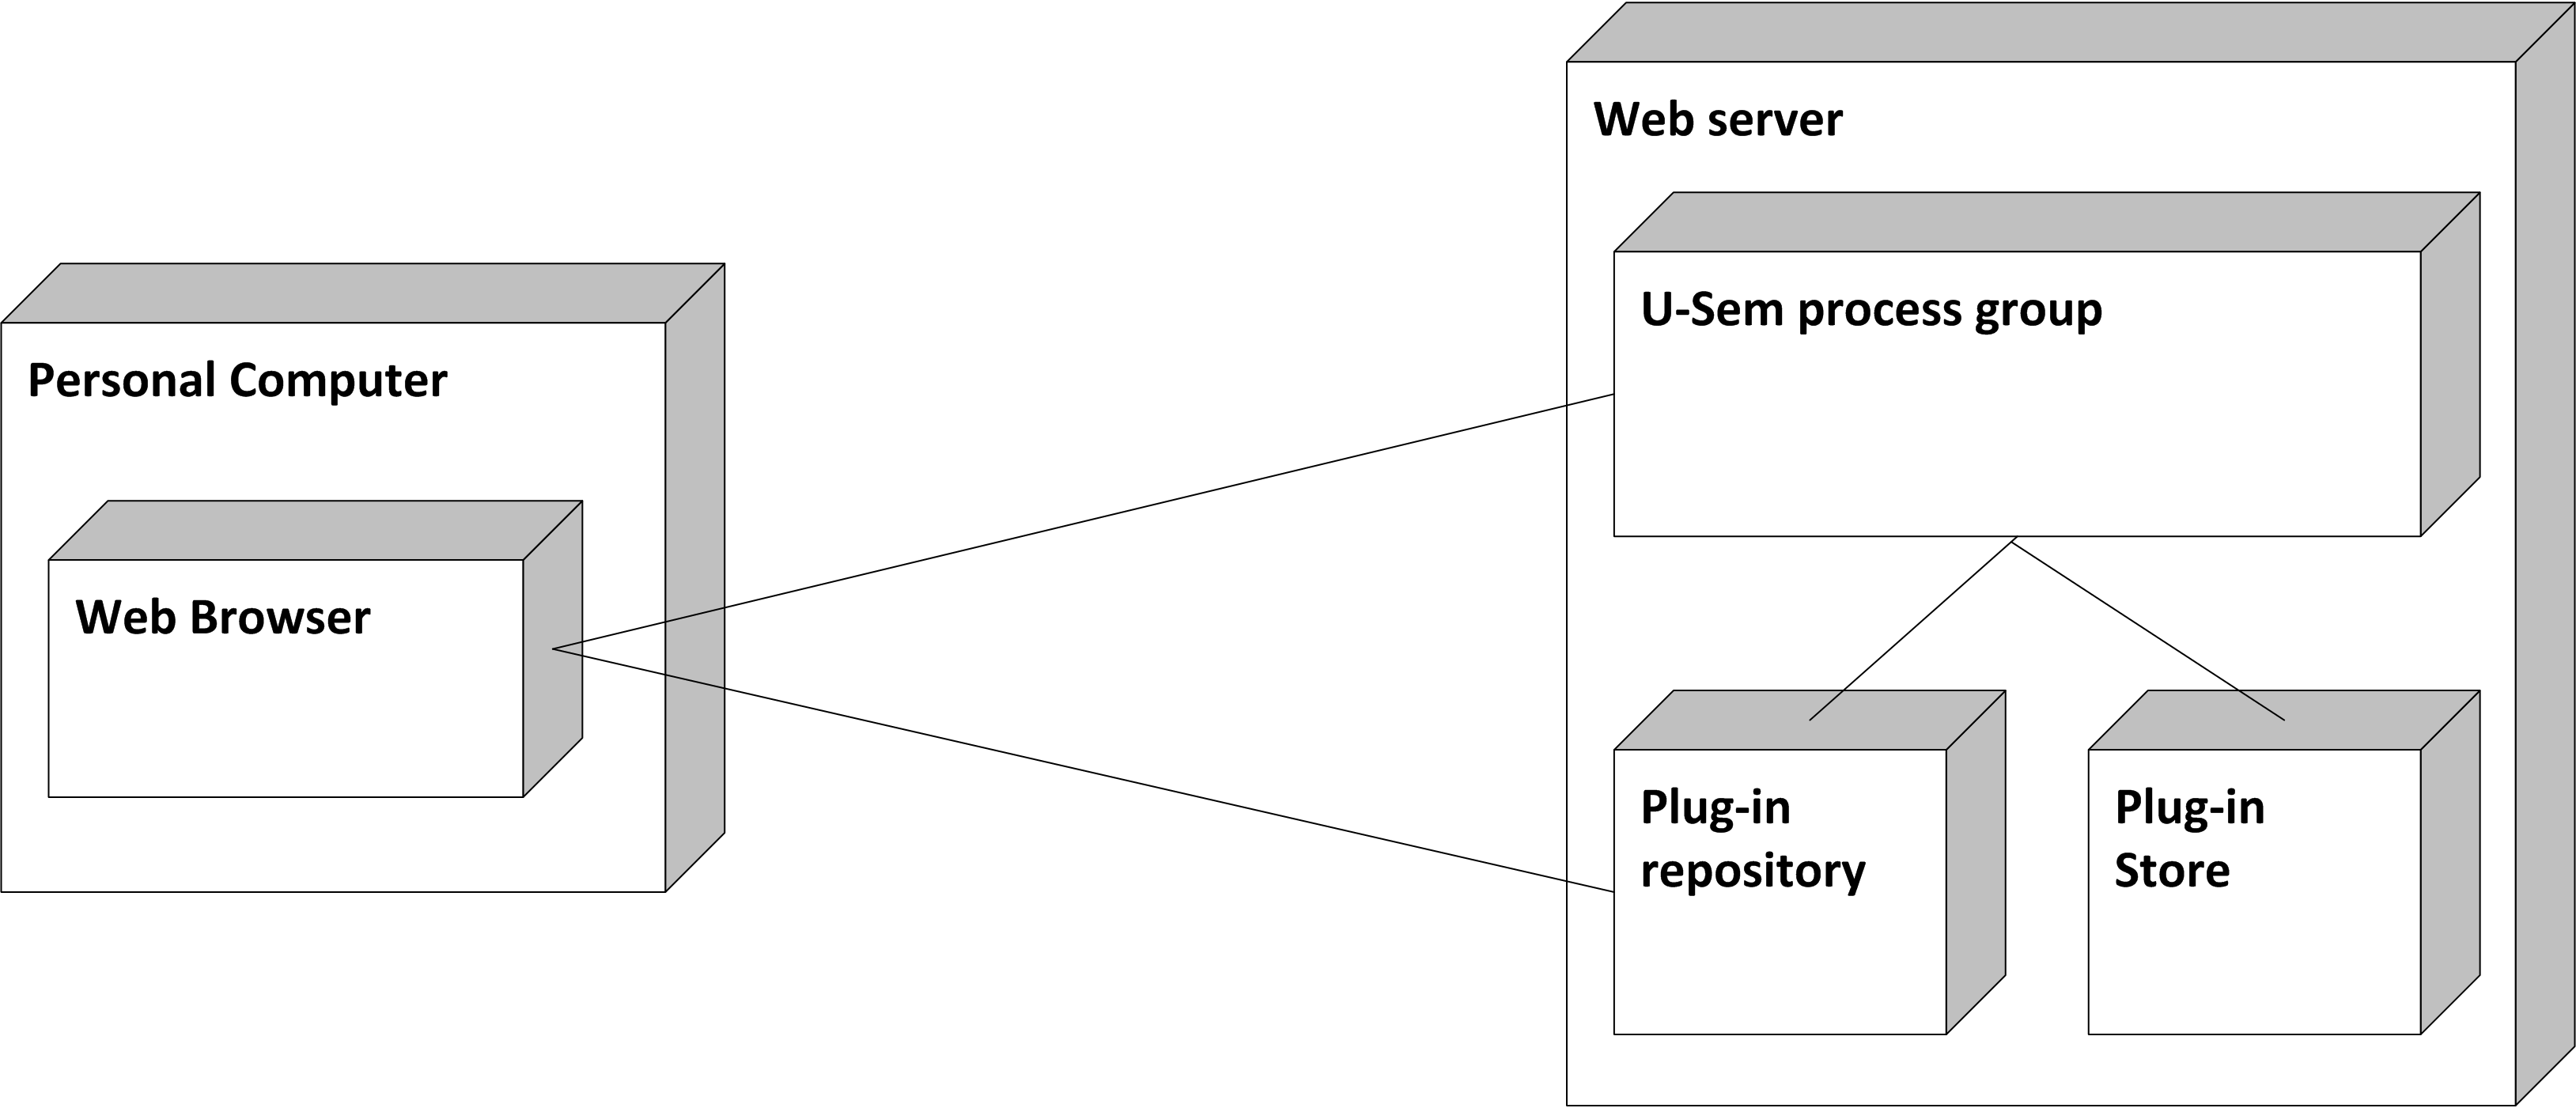
\includegraphics[scale=0.70]{plug-in/layers/simple_setup.png}
  \caption{Deployment diagram illustrating the simple setup of U-Sem}
  \label{simple_set}
\end{figure}

This deployment organization is illustrated on figure \ref{fig}. As you can see all component are deployed in the same web server on the same physical machine. We recommend this setup only for development and test purposes since it does not satisfy the performance, availability and security requirements. For production setup we recommend the one described in the next section.

\subsection{High Availability setup} 

This setup aims to cover the scenarios requiring high performance and high availability. Figure \ref{high_avail} provides the deployment diagram illustrating this setup.

The architecture defines a typical three tier organization. The presentation tier is represented by the user's web browsers and other client systems, the logical tier by the U-Sem backend process and the data storage tier by the plug-in store. In order to satisfy the scalability and availability requirements the logical and data storage tiers are distributed on multiple physical
devices. The backend process is replicated on several processing nodes to form a cluster. A load balancer situated between the cluster nodes and the client devices is responsible to distribute the load amongst the nodes. In case of a failure of a processing node, the load balancer no longer sends client request to it.

The database is also distributed. The storage is divided in several pieces based on the owner of the installed plug-ins. Then a node is assigned to each piece of data. Each node is responsible to store and provide access to the data of the assigned pieces. For extra security each device can be accompanied by another one which serves as a backup \textbf{Not in picture}. These is also a balancer between the logical and data tier which is responsible to redirect requests to the data node that is responsible for the data for the required user. Additionally, in case of a failure of a data node the load balancer is responsible to start sending request to its backup node and thus cause little times of unavailability.

In order to satisfy the security requirements, all communications are managed by firewalls placed before the load balancers. For clarity reasons they(the firewalls and load balancers) are displayed in the same components in the model but they can also be deployed on different processing units as well.


\begin{figure}[h!]
  \centering
  	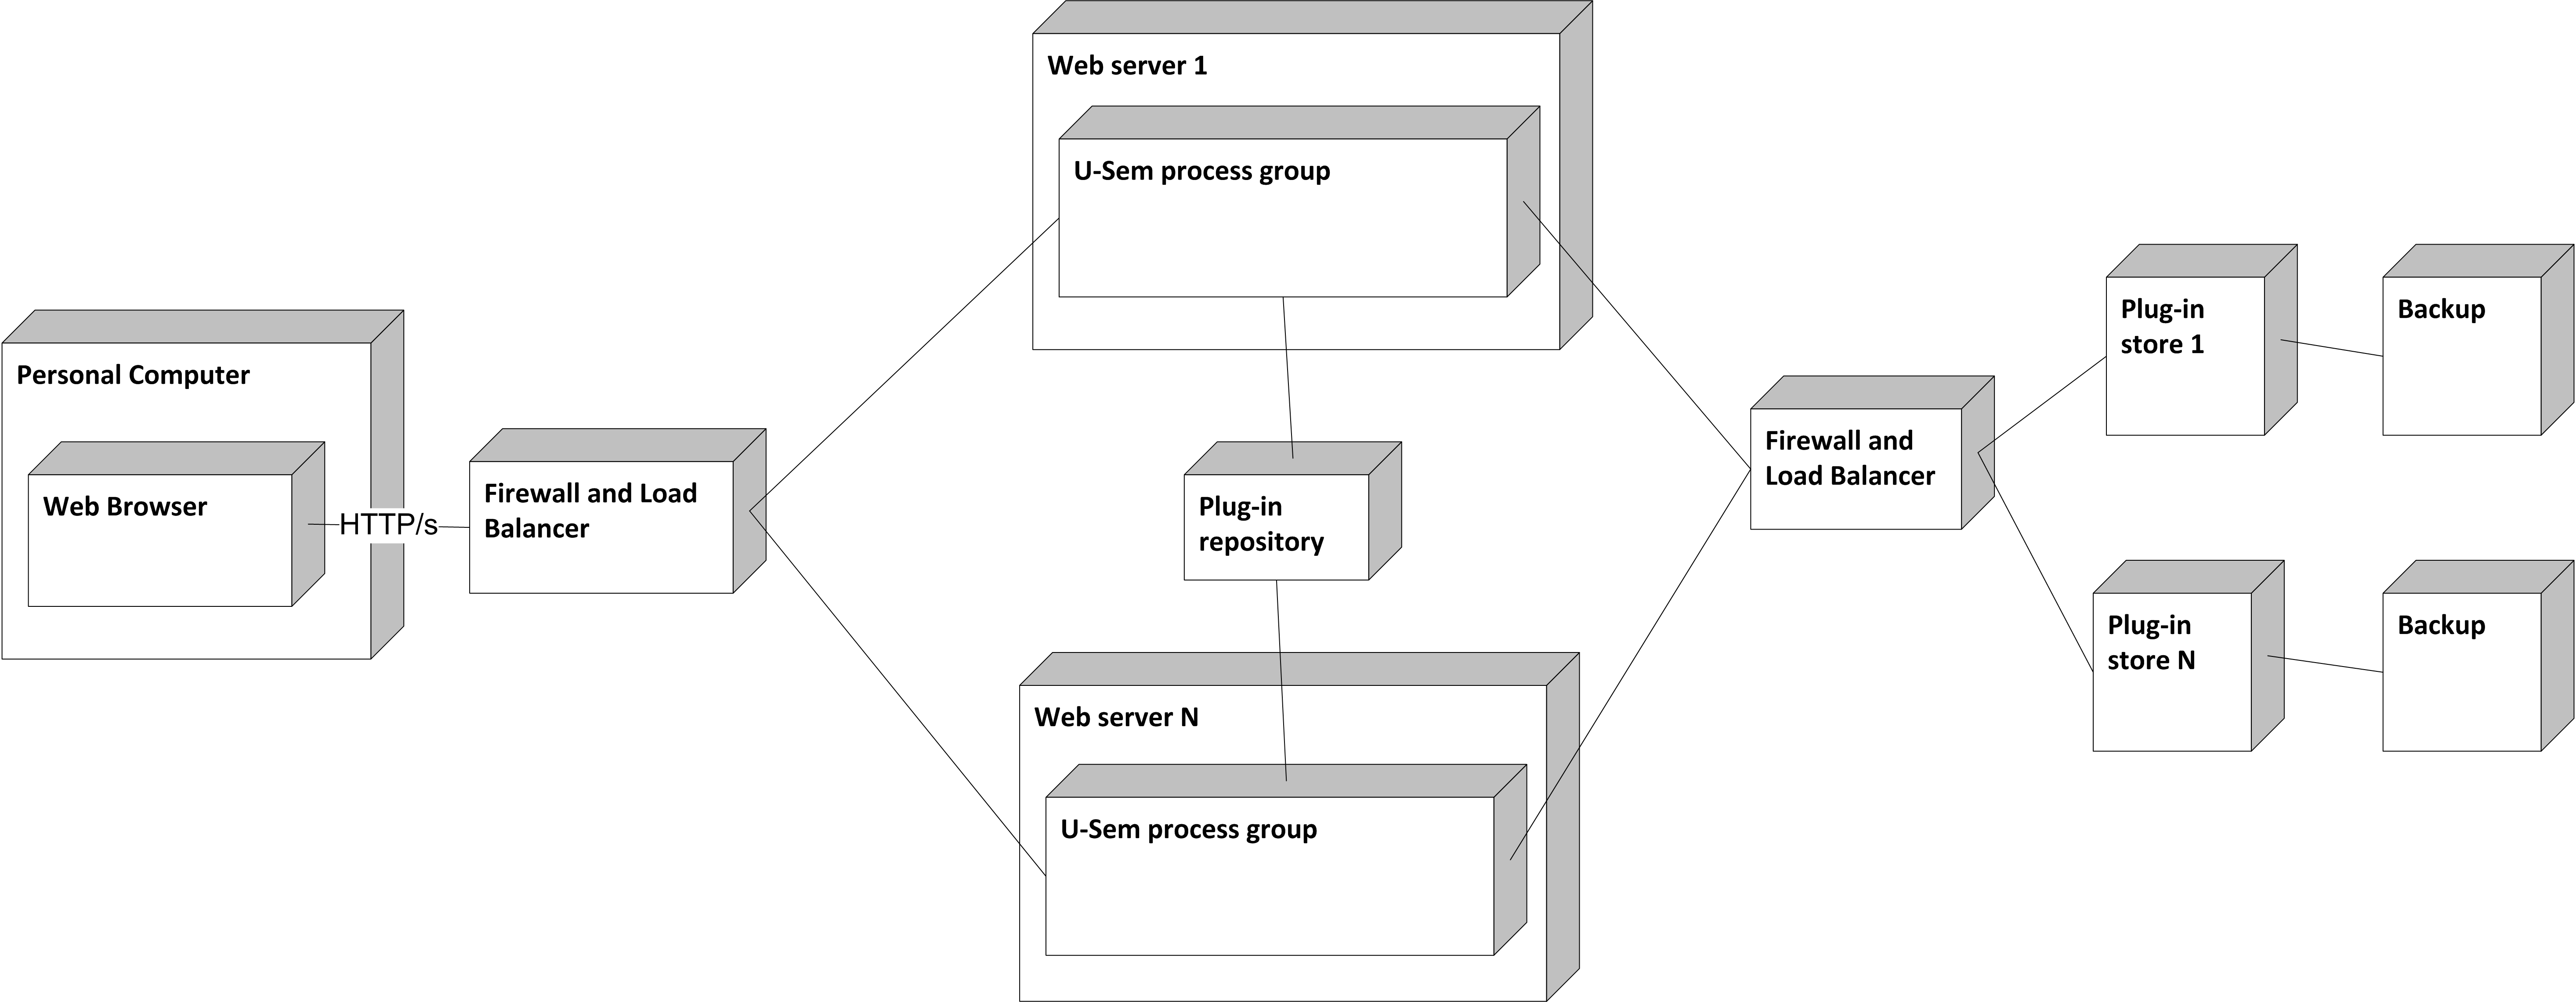
\includegraphics[scale=0.70]{plug-in/layers/high_setup.png}
  \caption{Deployment diagram illustrating the high availability setup of U-Sem}
  \label{high_avail}
\end{figure}

\section{Implementation}
\label{sec:impl}

In order to prove the applicabilities and capabilities of the system we actually implemented it. This section covers the most interesting steps performed during the implementation of the system.

First, we had to choose which OSGI implementation to use. Nowadays there are several vendors that provide implementations. The most popular are: Equinox, Felix and Knopflerfish. Theoretically, they all strictly implement the OSGI standard and therefore there should be little difference. However, we choose Equinox because it seemed more matured and more widely used then the others. Moreover, Equinox is highly integrated in the Eclipse IDE. This enables scientist to use the out-of-the box functionality for creating plug-ins in Eclipse.

Secondly, we had to decide the points where U-Sem can be extendend by providing custom functionality from plug-ins. At this point we identified that scientist has to be able to provide custom rdf gears functions and workflows. As explained earlier, in OSGI this points are represented as java interfaces. For custom functions we use the \textit{RGLFunction} class. The situation with the workflows was more complicated since they are represented as resource(xml) files. OSGI does not provide direct way for providing custom resource files from plug-ins. In order to overcome this problem we identified new class called \textit{WorkflowTemplate} which acts as a bridge and enables the workflow engine and other components to access workfow files provided by custom plug-ins.

\begin{figure}[h!]
  \centering
  	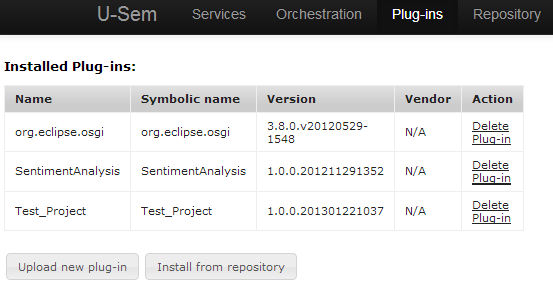
\includegraphics[scale=0.70]{plug-in/ui/list.png}
  \caption{User interface for plug-in management.}
  \label{list_ui}
\end{figure}

Next, we provided a very simple implementation of a plug-in repository. It represents a simple web application which stores the plug-in locally into the file system of the web server where it is deployed. The implementation provides resentful api for retrieving the list of available plug-ins and provide the contents of a selected plug-in. We also implemented very simple user interface which enables scientists to upload their plug-ins. 


\begin{figure}[h!]
  \centering
  	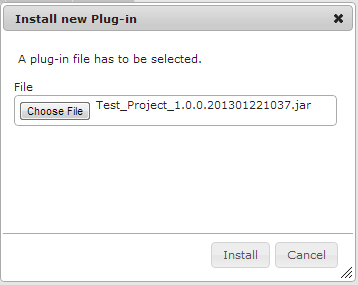
\includegraphics[scale=0.6]{plug-in/ui/upload.png}
  \caption{User interface for uploading and installing plug-ins in U-Sem.}
  \label{upload_ui}
\end{figure}

We continued by implementing all the components described in the architecture of U-Sem. In order to implement the end points(user interface) we used the JQuery and Bootstrap. Figure \ref{list_ui} represents the end point for viewing all installed plug-ins. Detailed information about all plug-ins is represented in the table. Each row has a "Delete" button which provides access to the functionality for removing plug-ins. At the bottom of the view there are two buttons that lead to the endpoints for uploading a plug-in illustrated in figure \ref{upload_ui} and the endpoint for browsing and installing functionality from the repository illustrated in figure \ref{repo_ui}.

\begin{figure}[h!]
  \centering
  	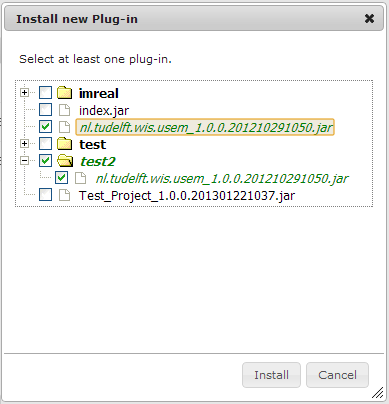
\includegraphics[scale=0.6]{plug-in/ui/repo.png}
  \caption{User interface for browsing and installing plug-ins from the plug-in repository.}
  \label{repo_ui}
\end{figure}

At the end we constructed a Maven build script that packs all source files into components(war files) that can be directly deployed to a web server. The entire system is composed in the following deployable files:
\begin{itemize}
	\item \textit{rdfgears.war} providing the workflow engine.
	\item \textit{pluginmanagement.war} providing the functionality for managing plug-ins.
	\item \textit{localPluginRepo.war} providing the implementation of the simple plug-in repository.
\end{itemize}

\section{Evaluation}
\label{sec:eval}

After successfully implementing the system we wanted to validate that the system complies with all functional and non-functional requirements discussed at the beginning of this chapter. 

\subsection{Functional requirements}

In order to validate the functional requirements we performed sevaral experiments and performed each of the defined scenarious.
 
Initially we had to build a component that encapsulates all functionality needed to perform the "Sentiment analysis" service. This functionality is currently hardcoded into the workflow engine outside. We used the already existing tools in Eclipse IDE to create the new plug-in. We removed all functionality and resource files from the workflow engine and put them into the newly created plug-in. The only additional thing that we had to do was to register the provided functionality. In Equinox this is done in the \textbf{Application} class. At the end we exported the plug-in into a traditional java jar file.

After we had built the plug-in we tried to execute each of the functional scenarios. Using the user interface we were able to plug in and use the components provided by the plug-in. We were able to view the installed plug-in in the management user interface and we were also able to successfully remove it from the system. At the end we were also able to share and install the plug in through the plug-in repository. All these proved that all functional requirements has been accomudated by the architecture and implementation of U-Sem.


\subsection{Non-functional requirements}

We believe that the proposed architecture will also satisfy the nonfunctional requirements of the system for the following reasons:

\begin{itemize}

\item \textit{Performance} - In each phase the user requests are distributed between several nodes which in the case of many users using the system makes it effective and reduces the response time.

\item \textit{Availability} - All operations are performed by clusters which means that in case of hardware or software failure of a cluster node the other nodes will continue to operate and the entire system will continue to be available. Additionally, availability in case of a storage node failure is ensured by redirecting all requests to its backup. Cluster nodes can also be placed in different physical locations to handle situation where an accident(e.g. network or electrical failure) in one data center can cause all devices to fail. Additionally, load balancers can be considered as a single points of failure. In order to overcome this problem we provide also clusters of load balancers and enable DNS load balancing.\textbf{more about dns}

\item \textit{Scalability} - One of the important requirements is that the system has to be able to gradually scale for supporting more users  by just adding new hardware components. This structure satisfies this requirement because in order to scale one should just add new nodes to the backend cluster, add new nodes to the database clusters. The system can be scaled up to the point where each workflow is executed by different node and the plug-ins for each scientist are stored on a different storage node.

\item \textit{Security} - The connection between the user and the backend can be encrypted(HTTPS) so that data transition is protected. The system's communication channels are also secured by firewalls. Also each storage node is backed up in case a device fails.

\end{itemize}


\section{Limitations and Future Work}
\label{sec:limits}

We have identified two types of limitations concerning U-Sem. The first one are the limitation inharited from the usage of OSGI. The second one concerns the rest of the U-Sem's architecture.

Most of the limitations concerning OSGI originate from the potential vulnerabilities of running external code which the security mechanism fails to fully address. The authors of \cite{Parrend} have studied in details the potential vulnerabilities of OSGI. These vulnerabilities cab be grouped into the following categories :

\begin{itemize}

	\item \textit{Vulnerabilities on operating system level} - This kind of vulnerabilities are due to the possibility that a plug-in runs native code either inside the JVM process or as a separate process. These vulnerabilities are enabled by JNI.
	
	\item \textit{Vulnarabilities on OSGi platform level} - This kind of vulnerabilities are related to weaknesses in the OSGi run-time. \cite{Parrend} suggests an approach for overcoming them by adding security checks in the OSGi implementation.
	
	\item \textit{Vulnarabilities on JVM level} - This vulnerabilities can be further divided into categories \cite{Geoffray}: 
	
	\begin{itemize}
		\item \textit{lack of isolation} - In the JVM \textit{java.lang.Class} objects and static variables are shared by all plug-ins. A malicious bundle can interfere with the execution of other bundles by altering static variables or obtaining lock on shared objects.
		
		\item \textit{lack of resource accounting} - In OSGI each plug-in is loaded with a separate class loader. However, JVM does not perform resource monitoring on a per class loader basis. Therefore, in case of the overuse of resources(CPU, memory), it is impossible to identify the faulty bundle and stop its execution.
		
		\item \textit{failure to terminate a bundle} -  If the system recognizes a bundle as misbehaving and wants to stop its
execution it might fail if methods of the bundle are being executed. Additionally, a malicious code can run an infinite loop in the Java \textit{finalize} method and thus prevent memory reclamation.
		
	\end{itemize}
	
	\cite{Geoffray} proposed and approach for overcoming these vulnerabilities. They have designed I-JVM, an extantion of the Java Virtual Machine which provides functionality for component isolation and termination in OSGi.
	
\end{itemize}

At this point U-Sem is aimed to be used by scientists of from single organization. Therefore, the components will only be reused within the organization which limits any external person from plug-in code into the system. Exploitation of these vulnerabilities on purpose is not so likely. Therefore, this limitation does not present significant threat to U-Sem. However, if in future the application U-Sem is to be extended to enable access to unverified scientists these vulnerabilities has to be removed. 

Another limitation of the architecture is defined by the fact that all components are reloaded again before each execution of a workflow. This is done for synchronization purposes if the installed plug-ins are changed. Even though it might be considered minute for most scenarios it can cause reduced performance in case many different workflows has to be executed in short amount of time. In future this limitation can be fixed by establishing communication mehanism between the workfow and plug-in management components. In this way when a change is made to the plug-ins a the workflow engine marks the loaded components as dirty and only then they are reloaded before the execution of the next workflow. not loading every time plug-ins. use cashe or communication between processes. \cite{Nikolov} also proposes approach for reducing the time needed to reload the components in OSGI.

\begin{thebibliography}{99}

\bibitem{Pour} G. Pour, Component-Based Software Development Approach: New Opportunities and Challenges, Proceedings Technology of Object-Oriented Languages, 1998. TOOLS 26., pp. 375-383.

\bibitem{Pour1}  G. Pour,  Enterprise JavaBeans,  JavaBeans and XML Expanding the Possibilities for Web-Based Enterprise Application Development,  Proceedings Technology of Object-Oriented Languages and Systems, 1999, TOOLS 31, pp.282-291.

\bibitem{Pour2} G.Pour, M. Griss, J. Favaro, Making the Transition to Component-Based Enterprise Software Development: Overcoming the Obstacles - Patterns for Success, Proceedings of Technology of Object-Oriented Languages and systems, 1999, pp.419 - 419.

\bibitem{Parnas} D. L. Parnas. On the criteria to be used in decomposing systems into modules. Communications of the ACM, 15(12):1053-1058, 1972.

\bibitem{Jifeng} H Jifeng, X Li, Z Liu, Component-based software engineering, Theoretical Aspects of Computing-ICTAC 2005

\bibitem{Cai} Cai, X. and Lyu, M.R. and Wong, K.F. and Ko, R, Component-based software engineering: technologies, development frameworks, and quality assurance schemes

\bibitem{Chen} Z Chen, Z Liu et al, Refinement and Verification in Component-Based Model Driven Design, Report of International Institute for Software Technology, 2007

\bibitem{Lau} Kung-Kiu Lau and Zheng Wang, Software Component Models

\bibitem{Bruneton} E. Bruneton, T. Coupaye, and J. Stefani, The Fractal Component Model, ObjectWeb Consortium, Technical Report Specification V2, 2003

\bibitem{OSGI} OSGi Alliance. http://www.osgi.org 

\bibitem{Andre} Andre L. C. Tavares, Marco Tulio Valente, A Gentle Introduction to OSGi

\bibitem{BPMN} Business Process Modeling Notation (BPMN) Specification, Final Adopted Specification. Technical report, Object Management Group (OMG), February 2006.

\bibitem{Decker} Decker, G. and Barros, A., Interaction modeling using BPMN, Business Process Management Workshops, 2008

\bibitem{Parrend} P. Parrend and S. Fr´enot. Security benchmarks of OSGi platforms: toward hardened OSGi. Software: Practice and Experience, 39(5):471-499, April 2009

\bibitem{Geoffray} Nicolas Geoffray, Gael Thomas, Gilles Muller, Pierre Parrend, Stephane Frenot, and Bertil Folliot: I-JVM: A Java Virtual Machine for Component Isolation in OSGi. In: DSN 2009

\bibitem{Nikolov} Vladimir Nikolov, Rüdiger Kapitza, Recoverable Class Loaders for a Fast Restart of
Java Applications

\bibitem{Srivastava} S Srivastava, M Hicks, Modular information hiding and type-safe linking for C, Software Engineering, IEEE Transactions on 2008

\bibitem{Eder} J Eder, G Kappel, M Schrefl, Coupling and cohesion in object-oriented systems, 1994
 

\end{thebibliography}